%%%%%%%%%%%%%%%%%%%%%%% file template.tex %%%%%%%%%%%%%%%%%%%%%%%%%
%
% This is a general template file for the LaTeX package SVJour3
% for Springer journals.          Springer Heidelberg 2010/09/16
%
% Copy it to a new file with a new name and use it as the basis
% for your article. Delete % signs as needed.
%
% This template includes a few options for different layouts and
% content for various journals. Please consult a previous issue of
% your journal as needed.
%
%%%%%%%%%%%%%%%%%%%%%%%%%%%%%%%%%%%%%%%%%%%%%%%%%%%%%%%%%%%%%%%%%%%
%
% First comes an example EPS file -- just ignore it and
% proceed on the \documentclass line
% your LaTeX will extract the file if required
\begin{filecontents*}{example.eps}
%!PS-Adobe-3.0 EPSF-3.0
%%BoundingBox: 19 19 221 221
%%CreationDate: Mon Sep 29 1997
%%Creator: programmed by hand (JK)
%%EndComments
gsave
newpath
  20 20 moveto
  20 220 lineto
  220 220 lineto
  220 20 lineto
closepath
2 setlinewidth
gsave
  .4 setgray fill
grestore
stroke
grestore
\end{filecontents*}
%
\RequirePackage{fix-cm}
%
%\documentclass{svjour3}                     % onecolumn (standard format)
%\documentclass[smallcondensed]{svjour3}     % onecolumn (ditto)
%\documentclass[smallextended]{svjour3}       % onecolumn (second format)
\documentclass[twocolumn]{svjour3}          % twocolumn
%
\smartqed  % flush right qed marks, e.g. at end of proof

\usepackage{microtype}
\usepackage{mathptmx}      % use Times fonts if available on your TeX system
\usepackage{amsmath, amssymb}
\usepackage{graphicx}
\usepackage{caption, subcaption}
\usepackage{threeparttable, booktabs}
\usepackage{cite}
\usepackage[misc]{ifsym}

%url
\usepackage{xurl}
\usepackage{hyperref}

%table
\usepackage{booktabs}
\usepackage{multirow}

%color
\usepackage{xcolor}
\newcommand{\pos}{\textcolor{green!70!black}{Positive}}
\newcommand{\nega}{\textcolor{red}{Negative}}

%code
\usepackage[linesnumbered,ruled,vlined]{algorithm2e}
\usepackage{algpseudocode}
%personal defintion
% \theoremstyle{remark}
\newtheorem{constraint}{Constraint}

\setlength{\emergencystretch}{3em}
% \newtheorem{definition}{Definition}
% \newtheorem{lemma}{lemma}
%%
%
% insert here the call for the packages your document requires
%\usepackage{latexsym}
% etc.
%
% please place your own definitions here and don't use \def but
% \newcommand{}{}
%
% Insert the name of "your journal" with
% \journalname{The VLDB Journal}

% for preprint
\journalname{Preprint}
\makeatletter
\def\makeheadbox{\relax}
\makeatother
%
\begin{document}

\title{LMG Index: A Robust and Efficient Learned Index Framework for Multi-Dimensional Performance Balance}
% \subtitle{Do you have a subtitle?\\ If so, write it here}

%\titlerunning{Short form of title}        % if too long for running head

\author{Yuzhen Chen \textsuperscript{1}\and
        Bin Yao \textsuperscript{1}
}

%\authorrunning{Short form of author list} % if too long for running head

\institute{
        \Letter Bin Yao \at
        \email{yaobin@cs.sjtu.edu.cn}   
        \and
        Yuzhen Chen \at
        \email{chenyz-sjtu@sjtu.edu.cn}
        \at
        {1} Shanghai Jiao Tong University, Shanghai, China 
}

\date{Received: date / Accepted: date}
% The correct dates will be entered by the editor


\maketitle

\begin{abstract}
Index structures are fundamental for efficient query processing on large-scale datasets. Learned indexes model the indexing process as a prediction problem to overcome the inherent trade-offs of traditional indexes. However, most existing learned indexes optimize only for limited objectives like query latency or space usage, neglecting other practical evaluation dimensions such as update efficiency and stability. Moreover, many learned indexes rely on assumptions about data distributions or workloads, lacking theoretical guarantees when facing unknown or evolving scenarios, which limits their generality in real-world systems.

In this paper, we propose LMG, a robust and efficient learned index framework designed for multi-dimensional performance balance. LMG integrates a decoupled routing structure with theoretical $O(1)$ complexity for fixed key types and an optimal error threshold training algorithm that approaches $O(1)$ overhead in practice. Furthermore, the framework enhances query performance by optimizing gap allocation. Extensive evaluations show that our framework achieves competitive or leading performance across all key evaluation dimensions, including bulk loading (up to 7.55$\times$ faster), point queries (up to 1.68$\times$ faster), range queries (up to 11.41$\times$ faster), and mixed read-write throughput (up to 3.50$\times$ faster). Furthermore, LMG ensures robust long-term stability and high space efficiency (up to 6.26$\times$ smaller footprint). These results demonstrate that LMG significantly mitigates the multi-dimensional performance trade-offs often observed in state-of-the-art approaches, offering a balanced and efficient framework.

\keywords{Learned index \and Robust framework \and Data access}
% \PACS{PACS code1 \and PACS code2 \and more}
% \subclass{MSC code1 \and MSC code2 \and more}
\end{abstract}

\section{Introduction}
\label{sec:intro}
The rapid development of information technology has resulted in an enormous amount of data, posing significant challenges to data management systems \cite{bigdata16}. Indexes are vital components that enhance query performance by avoiding exhaustive searches. Traditional indexes \cite{btree06, btree11, bwtree13, dynamichash98, hash16, lsmtree96, lsmtree17, remix21, adaptive18, adaptive22}, such as B+Tree, do not take full advantage of data distributions, leading to inefficiencies caused by pointer chasing and cache misses \cite{learned23}. Learned indexes \cite{case18}, proposed in recent years, regard index as a model of data distribution, and makes proper use of this model to improve query efficiency and reduce index size.

In recent years, learned indexes have emerged as a compelling alternative to traditional structures by treating the task of locating a record as a prediction problem. However, accurate position prediction is extremely difficult and expensive, instead, most learned indexes predict within an error threshold, then perform a bounded search around predicted position to locate the true position. To keep both training and prediction costs low, they employ simple models, such as linear model or a single-layer neural network. Moreover, to improve overall accuracy and reduce correction overhead, the data is partitioned into multiple segments, each trained with its own model so as to capture local distributions with high precision. This segmented modeling both raises prediction accuracy and enhances scalability, enabling learned indexes to handle large, complex datasets. Empirical studies \cite{sosd20} have shown that even a simple piecewise linear model works effectively on the majority of real-world datasets. Accordingly, most existing learned indexes \cite{pgm20, radixspline20, fiting-tree19, alex20, madex20, coax23, swix24, disklearned24} adopt piecewise linear regression as their prediction backbone.

Despite these gains, some evaluations \cite{sosd20, micro22, gre22, learned23} have shown that existing learned indexes still have a series of flaws. For example, \cite{case18, plex21, towards21} is only suitable for read-only workloads; \cite{xindex20, lipp21, finedex21, chameleon24} deliver excellent point queries throughput but suffer on range queries; \cite{pgm20} performs well after bulk loading but lack stability after updates; \cite{lipp21} achieves efficient queries and updates, but incur high space usage; \cite{alex20, swix24} impose slow bulk‐load times. Critically, most proposals focus on optimizing only one or two metrics at a time, making it difficult to achieve a multidimensional trade‑off that outperforms the classic B+Tree. This gap leaves learned indexes largely experimental: selecting the appropriate index for an unknown or evolving workload is itself a challenge. As a result, learned indexes struggle to gain traction in practical, real‑world settings.

To address these limitations, we propose LMIndex, a foundational structure optimized for query and space efficiency, and its variant LMG, which employs localized gap allocation to absorb dynamic updates and ultimately achieve multi-dimensional performance balance. Their design stems from the optimization of two fundamental indexing phases: (1) the segment index step, which locates the appropriate data segment. To guarantee structural robustness under dynamic workloads, this top-layer structure needs to maintain a small memory footprint, execute theoretical $O(1)$ routing, and eliminate cascading maintenance overheads. (2) the localized correction step, which searches within the target segment to find the exact record position. To sustain high-speed retrievals without sacrificing overall system balance, this process demands lower prediction errors and optimized local search algorithms. Concretely, LMIndex and LMG meticulously co-design the routing logic and local correction mechanisms to navigate inherent structural trade-offs, leading to the following contributions:

% \textbf{(1) A robust, spatio-temporal efficient segment index structure.} 
% We introduce the Linear Map (LM), an internal structure designed for indexing segments that maintains robust efficiency across dynamic workloads and diverse datasets. In practice, given a fixed key type, the LM achieves $O(1)$ complexity for both queries and updates. Empirically, it incurs an average space overhead of only 4\% in our experiments.

\textbf{(1) Robust and Efficient Segment Index Structure.} To optimize the segment index step, we introduce Linear Map (LM). Compared to other segment index structures, LM eliminates the need for complex model training. Instead, it utilizes a deterministic mapping approach that flexibly and efficiently adapts to changes in the underlying segment distribution. Consequently, given a fixed key type, LM achieves $O(1)$ time complexity for both queries and dynamic updates. Empirically, it maintains robust performance across diverse datasets while incurring an average space overhead of only 4\%.

\textbf{(2) Optimal Error Threshold Compression Algorithm for Local Correction.} To optimize the local correction step, we introduce the Optimal Error Threshold Algorithm (OETA). Compared to the least squares method, OETA minimizes the maximum prediction error within each segment while achieving performance that is independent of distribution and nearly constant in time. Furthermore, we demonstrate that binary search (BS) outperforms exponential search (ES) on complex distributions. OETA accelerates BS, enabling it to match the performance of exponential search even on highly linear distributions.

% \textbf{(3) Robust and Efficient Framework for Multi-Dimensional Balance.} By integrating the LM structure with the OETA algorithm, we first construct LMIndex, a foundational structure strictly optimized for read efficiency and compact space utilization. Building upon this baseline, we develop LMG, an write-optimized variant employing a gapped array coupled with a novel gap allocation strategy. Consequently, LMG mitigates the severe performance trade-offs inherent in state-of-the-art baselines, delivering a highly robust and efficient framework that maintains performance stability and competitive read/write throughput across all evaluation dimensions.

\textbf{(3) Robust and Efficient Framework for Multi-Dimensional Balance.} By integrating the LM structure with the OETA algorithm, we first construct LMIndex, a foundational learned index framework employing a dense data layout. To unleash its potential in dynamic environments, we further develop LMG, a variant employing a gapped data layout and a novel gap allocation strategy. LMG mitigates the performance trade-offs inherent in state-of-the-art baselines, delivering a highly robust and efficient framework that maintains performance stability and competitive read/write throughput across all evaluation dimensions.

The remainder of this paper is organized as follows. Section \ref{sec:back&moti} describes the background and motivation. Section \ref{sec:overview} provides an overview of the overall design of LMIndex and LMG, including basic operations. Section \ref{sec:lm} introduces the Linear Map in detail. Section \ref{sec:single-model} introduces Optimal Error Threshold Algorithm. Section \ref{sec:evaluation} presents experimental analysis. Section \ref{sec:extend} explores the extensibility of our framework to broader database operations. Section \ref{sec:rel-work} reviews related work in the field. Finally, Section \ref{sec:conclusions} concludes the paper.

\section{Background and Motivation}
\label{sec:back&moti}
\subsection{The Idea of Learned Index}
The concept of learned indexes is inspired by machine learning: an index can be viewed as a model that maps keys to storage addresses, and building an index is analogous to training that model\cite{case18}. Concretely, the index model is the empirical cumulative distribution function (ECDF) of dataset, so the core idea of learned indexing is to construct models that fit the ECDF. In practice, however, fitting a complex real-world ECDF with a single global model is difficult and brittle under distribution shifts. Therefore, most practical learned index designs adopt multi-model hierarchies: an upper layer directs queries to leaf layer models, which are typically piecewise functions that provide more accurate local fits. In addition, indexes applies the final “last-mile” search corrects any residual prediction error when necessary.

One representative realization of this multi-model hierarchies is the Recursive Model Index (RMI) framework \cite{case18}. In RMI, each layer consists of multiple models, where a higher-level model selects the next-layer model, and the leaf-layer model predicts the position within its local range, followed by a correction search to find the exact key. Error correction in multi-model hierarchies can be performed either at internal/leaf nodes \cite{pgm20, xindex20, finedex21} or only at leaf nodes \cite{case18, alex20}; all corrections introduce runtime overhead. LMIndex achieves perfect accuracy in internal node predictions, eliminating the need for internal node correction and its associated cost.

At the leaf level, learned indexes often adopt piecewise linear models due to their structural simplicity and sufficient fitting capability \cite{sosd20}. Constructing a piecewise linear function typically involves two phases: segmentation and training. Some indexes \cite{alex20, swix24, carmi22} perform segmentation using independent heuristics and then train per-segment models via least squares regression. An alternative family of approaches \cite{fiting-tree19, pgm20, bourbon20} follows an $\varepsilon$-constrained construction: during segmentation, an error threshold $\varepsilon$ is enforced so that each segment’s model satisfies the constraint:

\begin{constraint}[$\varepsilon$-constraint]
\label{cons:epsi}
    For all keys $k$ in a segment, have $|\hat{p}(k) - p(k)| \le \varepsilon$, where $\hat{p}(k)$ is the predicted position and $p(k)$ is the true position.
\end{constraint}

Several methods, including RS \cite{radixspline20} and LIPP \cite{lipp21}, use greedy one-pass segment generation algorithms to produce $\varepsilon$-constrained partitions efficiently. The PGM-Index \cite{pgm20} adapts the streaming algorithm from \cite{line81} to construct the optimal piecewise linear approximation model (Opt. PLA-model), which generates the minimum number of $\varepsilon$-constrained segments in one pass. Opt. PLA constructs, for each prospective segment, a convex region of slope–intercept pairs that satisfy the $\varepsilon$-constrain and simply chooses the central point as the model parameter.

% Compared with independent training strategies, $\varepsilon$-constrained approaches typically require only $O(n)$ time for segmentation, and part of training cost is implicitly embedded in the segmentation process, yielding higher construction efficiency. However, Opt. PLA-model focuses solely on optimal segmentation and does not optimize the training phase. LMIndex builds upon this foundation with the Optimal Error Threshold Algorithm (OETA), which computes model parameters with the minimum maximum error for each segment in constant time. Combined with binary search for final error correction, LMIndex adapts to the local distribution of each segment, thereby reducing correction overhead.

Compared to independent segmentation-then-train pipelines, $\varepsilon$-constrained approaches typically run in $O(n)$ time for segmentation, and the part of training cost is implicitly embedded in the segmentation process, yielding higher construction efficiency. However, Opt. PLA-model focuses solely on optimal segmentation and does not optimize the training phase. LMIndex builds upon this foundation with the Optimal Error Threshold Algorithm (OETA), which efficiently computes per-segment linear parameters that minimize the segment’s maximum prediction error. Combined with binary search for final error correction, OETA allows LMIndex to adapt each segment to its local distribution and significantly reduce last-mile correction overhead.

% \begin{table}
%   \caption{B+Tree vs. Learned indexes across six key dimensions}
%   \small
%   \begin{tabular}{lccccc}
%     \toprule
%      &\textbf{B+Tree}&\textbf{DPGM}&\textbf{ALEX}&\textbf{LIPP}&\textbf{FINEdex}\\
%     \midrule
%     \textbf{Bulk load} & $\triangle$ & $\triangle$ & $\times$ & $\times$ & $\times$\\
%     \textbf{Point query} & $\triangle$ & $\bigcirc$ & $\bigcirc$ & $\bigcirc$ & $\triangle$\\
%     \textbf{Range query} & $\triangle$ & $\triangle$ & $\triangle$ & $\times$ & $\times$\\
%     \textbf{Update} & $\triangle$ & $\bigcirc$ & $\times$ & $\triangle$ & $\triangle$\\
%     \textbf{Stability} & $\triangle$ & $\times$ & $\triangle$ & $\triangle$ & $\triangle$\\
%     \textbf{Space} & $\triangle$ & $\bigcirc$ & $\triangle$ & $\times$ & $\times$\\
%   \bottomrule
%   \label{tab:learnedVSbtree}
% \end{tabular}
% % \footnotesize{$\bigcirc$: good; $\triangle$: moderate; $\times$: poor.}
% \vspace{-8pt}
% \begin{tablenotes}
%     \small
%     \item \textbf{Compared to B+Tree:} $\bigcirc$: better; $\triangle$: similar; $\times$: worse.
%   \end{tablenotes}
% \end{table}

% \begin{table}
%  \centering
%   \caption{B+Tree vs. Learned indexes across six key dimensions}
%   \small
%   \begin{tabular}{lccccc}
%     \toprule
%      &\textbf{B+Tree}&\textbf{DPGM}&\textbf{ALEX}&\textbf{LIPP}&\textbf{FINEdex}\\
%     \midrule
%     \textbf{Bulk load} & $\triangle$ & $\triangle$ & $\times$ & $\times$ & $\times$\\
%     \textbf{Point query} & $\triangle$ & $\bigcirc$ & $\bigcirc$ & $\bigcirc$ & $\triangle$\\
%     \textbf{Range query} & $\triangle$ & $\triangle$ & $\triangle$ & $\times$ & $\times$\\
%     \textbf{Update} & $\triangle$ & $\bigcirc$ & $\times$ & $\triangle$ & $\triangle$\\
%     \textbf{Stability} & $\triangle$ & $\times$ & $\triangle$ & $\triangle$ & $\triangle$\\
%     \textbf{Space} & $\triangle$ & $\bigcirc$ & $\triangle$ & $\times$ & $\times$\\
%   \bottomrule
%   \label{tab:learnedVSbtree}
% \end{tabular}
% % \footnotesize{$\bigcirc$: good; $\triangle$: moderate; $\times$: poor.}
% \vspace{-8pt}
% \begin{tablenotes}
%     \small
%     \item \textbf{Compared to B+Tree:} $\bigcirc$: better; $\triangle$: similar; $\times$: worse.
%   \end{tablenotes}
% \end{table}

% \begin{table}
%   \centering
%   \caption{B+Tree vs. Learned indexes across five key dimensions}
%   \small
%   \begin{tabular}{lcccc}
%     \toprule
%       &\textbf{B+Tree}&\textbf{DPGM}&\textbf{ALEX}&\textbf{LIPP}\\
%     \midrule
%     \textbf{Bulk load} & $\triangle$ & $\triangle$ & $\times$ & $\times$\\
%     \textbf{Point query} & $\triangle$ & $\bigcirc$ & $\bigcirc$ & $\bigcirc$\\
%     \textbf{Range query} & $\triangle$ & $\triangle$ & $\triangle$ & $\times$\\
%     \textbf{Update} & $\triangle$ & $\bigcirc$ & $\times$ & $\triangle$\\
%     \textbf{Stability} & $\triangle$ & $\times$ & $\triangle$ & $\triangle$\\
%     \textbf{Space} & $\triangle$ & $\bigcirc$ & $\triangle$ & $\times$\\
%   \bottomrule
% \end{tabular}
% \label{tab:learnedVSbtree}
% % \footnotesize{$\bigcirc$: good; $\triangle$: moderate; $\times$: poor.}
% % \vspace{-4pt}
% \begin{tablenotes}
%     \small
%     \item \textbf{Compared to B+Tree:} $\bigcirc$: better; $\triangle$: similar; $\times$: worse.
%   \end{tablenotes}
% \end{table}

% \subsection{Learned Indexes vs. B+Tree}
% Learned indexes have attracted significant attention for their potential to exploit data distribution to accelerate query processing. Nevertheless, compared to the mature and widely adopted B+Tree, existing learned index designs invariably fall short in one or more critical dimensions. This discrepancy restricts their applicability as versatile indexes in practical database systems.

% Table \ref{tab:learnedVSbtree} summarizes the comparison among B+Tree, DPGM, ALEX, LIPP, and FINEdex across six key evaluation dimensions. All symbols represent performance comparisons against B+Tree. For example, $\bigcirc$ indicates better performance than B+Tree, while $\triangle$ denotes similar performance to B+Tree. All dimensions (except space) are evaluated in terms of latency. For Stability, we evaluate the deviation in read/write latency after updates. The results highlight that no existing learned index consistently outperforms B+Tree across all these dimensions. We briefly analyze the underlying reasons for these limitations below.

% \textbf{DPGM.} DPGM \cite{pgm20} extends the original read-only PGM-index by organizing data into sorted sets of exponentially increasing size, each independently indexed with a read-only PGM. New entries are inserted into the smallest set and trigger merges upon overflow, which involves retraining a static PGM for the merged set. While enabling updates, DPGM suffers from unstable query performance post-update: unlike B+Tree’s logically contiguous leaf data layout, DPGM disperses data across multiple sets, causing point queries to probe several models and range queries to merge partial results from each set, thus incurring higher latency and resource consumption.

% \textbf{ALEX.} ALEX \cite{alex20} segments data using a cost model involving complex sampling and computation, followed by $O(n)$-time least squares training per segment. Its construction demands multiple passes over data and maintains a complex cost model, whereas B+Tree can be bulk-loaded with one pass. Under heavy updates cause drastic changes in the data distribution, ALEX experiences frequent node splits and retraining, and pay further overhead to maintain the cost model. In contrast, B+Tree updates are less sensitive to data distribution and avoid the burden of model recalibration.

% \textbf{LIPP.} LIPP \cite{lipp21} eliminates correction both at internal and leaf nodes by ensuring perfect prediction. To prevent “last-mile” correction, it recursively partitions conflicting key sets and retrains models until each key is uniquely placed. This leads to high bulk loading cost on complex distributions due to repeated conflict resolution and retraining. And scattered data layouts of LIPP increase range query overhead compared to B+Tree’s linked leaf nodes. Additionally, LIPP’s conflict-driven model proliferation may cause large internal gaps and unpredictable space usage, especially on real-world skewed data, unlike B+Tree’s stable space footprint.

% \textbf{FINEdex.} FINEdex \cite{finedex21} employs the Learning Probe Algorithm (LPA) to adaptively train models and optimize layout, storing them in a SIMD-optimized B-Tree. LPA uses least squares fitting, probing whether appending a block exceeds an error threshold, and performing localized rollbacks if necessary. This LPA-based construction requires multiple data passes, thus incurring greater construction complexity compared to B+Tree’s one pass bulk load. For updates, LIPP employs an optional per-key “level bins” to absorb insertions. Although its fine-grained buffering can absorb more keys, it increases range query cost and space overhead.

% \textbf{Motivation.} As summarized above, existing learned indexes tend to trade off improvements in few metric for another, limiting their generality under unknown or dynamic workloads and data distributions. This gap motivates us to design a comprehensive learned index that achieves superiority compared to B+Tree across multiple key dimensions (including bulk load, point and range queries, updates, stability, and space usage), while simultaneously maintaining competitiveness with state-of-the-art learned indexes.

\begin{table*}[htbp]
\centering
\caption{Impact of Design Strategies on Key Evaluation Dimensions. Note that Negative/Positive denote relative impacts within the same main strategy. Unmarked entries depend on specific implementations (e.g., query performance of hybrid strategies depends on the additional structure).}
\label{tab:strategy_dimensions}
\renewcommand{\arraystretch}{1.3}
\begin{tabular}{ll cccccc}
\toprule
\textbf{Main Strategy} & \textbf{Sub-Strategy} & \textbf{Bulk Loading} & \textbf{Point Queries} & \textbf{Range Queries} & \textbf{Update} & \textbf{Stability} & \textbf{Space Usage} \\
\midrule

% 1. Model training strategies
\multirow{2}{*}{Model training} 
& Top-Down & \nega & \pos & & \nega & \nega &\\
& Bottom-Up & \pos & & & \pos & \nega &\\
\midrule

% 2. Segments indexing strategies
\multirow{2}{*}{Segments indexing} 
& RMI-style & & \pos & & \nega & \nega & \pos \\
& Hybrid & & & & \pos & \pos & \nega\\
\midrule

% 3. Error management strategies
\multirow{3}{*}{Error management} 
& All Node Error & & \nega & & & & \pos \\
& Leaf-only Error & \nega & \pos & & & & \\
& Zero Error & & \pos & \nega & & & \nega \\

\bottomrule
\end{tabular}
\end{table*}

\subsection{Design Strategy Analysis of Learned Index}
Although learned indexes demonstrate performance potentials exceeding traditional counterparts in specific scenarios, their robustness faces severe challenges under uncertain operating environments. Existing studies \cite{pgm20, lipp21} tend to highlight a small number of metrics (eg, lookup speeds) in specific scenarios, but their performance frequently decays when triggered by shifts in data distribution, hardware resource constraints, or workload fluctuations. The core pain point lies in the instability of performance or even unavailability (e.g. out of memory in some devices), which limits the potential for learned indexes to be widely deployed in practice.

The underlying cause of this fragility is that existing designs often pursue specialized optimization of single or few performance dimensions, neglecting the complex interference among different dimensions. Notably, the performance dimensions of an index, such as point query latency, space usage, and update latency, are not independent but tightly coupled. For instance, strategies that minimize point query latency to the extreme, such as LIPP \cite{lipp21}, incur a multiplicative expansion of the memory footprint compared to other baselines\cite{learned23}. This observation suggests that a lack of holistic consideration regarding these inter-dimensional trade-offs leads to the observed lack of robustness. Understanding the trade-offs of existing strategies is essential to enhance index robustness. Therefore, we present the following design strategies:

\subsubsection{Model Training Strategies}
In the context of model training paradigms, Top-Down and Bottom-Up strategies exhibit distinct trade-offs across multiple performance dimensions. (1) \textbf{Top-Down strategies} \cite{case18, alex20, swix24} treat the dataset as a whole and attempt to fit a global model. This method recursively partitions the dataset into subsets to improve precision of models. While this utilizes global distribution of the dataset to reduce random memory accesses and optimizes average read latency in static settings, the training process requires multiple passes over the full data, resulting in low efficiency during bulk loading. Furthermore, the advantages of this approach primarily stem from partitioning based on the perception of global distribution. Consequently, when the data distribution undergoes changes, either frequent cascading updates are required to maintain high efficiency, leading to significant update cost, or distribution drift is permitted, which results in a subsequent decline in query efficiency. (2) \textbf{Bottom-Up strategies} \cite{radixspline20, pgm20, finedex21}, represented by Piecewise Linear Approximation (PLA) \cite{pgm20}, greedily construct segments (i.e. data partitions containing the model) based on a strict maximum model prediction error threshold and build segment indexes upward from these segments. These methods are typically efficient for bulk loading, as they require only a single pass over the data. Furthermore, they remain insensitive to changes in the global distribution, given that the impact of insertions is usually confined to local regions. However, the fixed parameters of such methods (e.g. maximum error threshold) are immutable during construction, which may generate a large number of segments on skewed datasets. Furthermore, updates potentially exacerbate this increase in the segment count. Thus, segment indexing becomes critical and some indexing strategies may lead to severe degradation of query efficiency after updates \cite{pgm20, learned23}.

\subsubsection{Segments Indexing Strategies}
Consistent with the above, a segment is defined as a bottom data partition and its corresponding model (In context of B+Tree, it's leaf node). Similarly, in the design of indexing structures for managing segments, a significant conflict exists between structural flexibility and maintenance overhead. (1) \textbf{RMI-Style strategies} \cite{xindex20, chameleon24, sali23} index segments using models of varying precision. A request initially enters the lowest precision model and progressively predicts and transitions to the next layer of higher precision models until it is routed to the target segment. The advantage of this approach lies in the small memory footprint of model parameters and typically low prediction overhead. However, it faces a challenge in balancing precision and flexibility. High-precision models are tightly coupled with the data distribution, where structural modification operations (SMOs) may trigger cascading retraining and result in significant overhead. Conversely, models prioritizing flexibility permit prediction errors and rely on local correction, which compromises query efficiency. (2) \textbf{Hybrid strategies} employ additional structures or their model-integrated variants to locate segments, including B+Trees \cite{fiting-tree19, learnedkv24}, flat arrays \cite{swix24, uplif25}, hash tables \cite{lits24, lead26}, etc. The SMO of this approach generally exhibit less dependence on the data distribution, thereby partially mitigating the cascading retraining issues associated with previous methods. Furthermore, different underlying structures provide distinct advantages. For instance, B+Trees offer efficient construction alongside relatively balanced update and search performance, whereas hash tables support high-speed insertions and point queries. However, compared to RMI-Style strategies, hybrid approaches introduce additional space overhead. Furthermore, these designs inherit the specific limitations of their chosen structures, such as the search latency inherent in trees or the poor range query efficiency of hash tables.

\subsubsection{Error Management Strategies}
The error management strategy determines how the gap between the predicted position and the true position is bridged, triggering a triangular game among query latency, construction cost, and spatial continuity. Depending on the source of the error, it can be divided into three classes: (1) \textbf{All Node Error strategies} \cite{plex21, hlihp24} permits prediction inaccuracies across all nodes. This strategy benefits from simpler models, such as basic linear regression, and results in the minimal storage overhead for model parameters. However, error correction costs accumulate at every node along the query propagation path, which leads to reduced query efficiency. (2) \textbf{Leaf-only Error strategies} \cite{alex20, lits24, alt-index25} restricts prediction inaccuracies to leaf nodes (i.e., segment nodes), thereby reducing the frequency of error correction to $O(1)$ complexity and effectively decreasing query overhead. Achieving this strategy typically requires complex node splitting logic, which prolongs bulk loading time. Furthermore, certain implementations \cite{alex20} lack theoretical constraints on the maximum error of leaf nodes. (3) \textbf{Zero Error strategies} like LIPP \cite{lipp21} force physical positions to match predictions. While this eliminates correction search and optimizes point queries, it necessitates reserving massive empty slots. This results in spatial inflation and memory discontinuity, which severely degrades the performance of range queries.

In summary, most existing learned indexes represent compromises on specific performance metrics under limited assumptions. This design philosophy limits their generality in complex, dynamic environments. To this end, our goal is not to pursue single-point extremism but to design a robust and efficient framework. We aim to coordinate the aforementioned conflicts to achieve an optimal balance among critical performance dimensions, including bulk loading efficiency, point and range query performance, update throughput, stability, and space usage.

\subsection{Strategies Selection for Multi-dimensional Performance Balance and Efficiency}
As summarized in Table \ref{tab:strategy_dimensions}, existing strategies inherently incur trade-offs across different evaluation dimensions. With the objective of multi-dimensional comprehensive optimization, the key idea for selecting strategies is to exploit their inherent strengths while mitigating their respective weaknesses. Based on this systematic analysis, we identify two core philosophies: \textbf{(1) simple and universal strategies generally outperform complex designs tailored for single-dimensional gains; (2) Allowing constrained deviations or limited chaos is often more effective across multi-dimensions than strategies of absolute restriction or complete freedom.} Specifically, we select:

\textbf{Model training strategies.} We adopt Bottom-Up strategies. Compared to Top-Down strategies, which suffer from low bulk loading efficiency due to multiple data scans and high sensitivity to distribution drift, Bottom-Up strategies are more simple and universal. This approach requires only a single pass to complete construction, and its greedy algorithm offers the advantages of high efficiency and local decoupling. Furthermore, to address the issue of immutable preset error thresholds, we propose the OETA algorithm to compress the threshold of each segment to its minimum. To overcome the potential drawback of excessive segment generation, we introduce a novel segment indexing strategy that ensures the theoretical maximum routing length remains strictly bounded and small.

\textbf{Segments indexing strategies.} We adopt Hybrid strategies. Specifically, we design a novel flat/tree-like hybrid structure named Linear Map (LM) to index segments and mitigate the inherent drawbacks of Bottom-Up strategies. Compared to traditional structures, LM exploits segment distribution information. When the key type is fixed, the theoretical complexity of both queries and updates remains $O(1)$. The core model of this structure is essentially a derivation of the segments, enabling LM to achieve precise routing to target segment without the need for model training. This ensures simultaneous efficiency in both construction and query execution. Furthermore, experimental results demonstrate that its space consumption is second only to RMI-Style strategies.

\textbf{Error management strategies.} We adopt Leaf-only Error strategies. In practice, error management strategies can be viewed as a spatio-temporal trade-off. While the All Node Error strategies maximizes space savings at the expense of query efficiency, the Zero Error strategies achieves theoretically optimal query efficiency but it needs to allocate empty slots in advance. This requirement leads to both severe space inflation and degraded performance for range queries. The Leaf-only Error strategy represents a compromise between these two extremes. By incorporating OETA to ensure that leaf node errors remain controlled, it avoids space wastage while simultaneously maintaining high performance for both point and range queries. Furthermore, we design a gaps allocation strategy and hybrid search to further reduce the cost of error correction within leaf nodes.


% \section{Piecewise Linear Model}
% \label{sec:plm}
% % Let $A$ be a sorted array of $n$ keys, $A=\{(key_0,pos_0), ... , (key_i,pos_i), \\ ..., (key_{n-1},pos_{n-1})\}$ and let $\varepsilon \ge 1$ be an integer. A PLM $P=(A, S, \varepsilon)$, where $S = \{s_0, s_1, ... , s_{m-1}\}$ contains $m$ segments and $\varepsilon$ is an error threshold. $S$ is a sorted segment set, where $s_i$ represents a segment. $P$ is considered as the set of $s_i$ built on $A$ with parameter $\varepsilon$.
% As discussed in Section \ref{sec:intro}, we focus on PLM with a maximum error constraint. Let $A$ be a sorted array of $n$ keys, $A=\{(key_0,pos_0), ... , \\ (key_i,pos_i), ..., (key_{n-1},pos_{n-1})\}$, and let $\varepsilon \ge 1$ be an integer. A PLM $P=(A, S, \varepsilon)$, where $S = \{s_0, s_1, ... , s_{m-1}\}$ contains $m$ segments $s_i$, and $\varepsilon$ is an error threshold. $P$ is considered as the set of $s_i$ built on $A$ with parameter $\varepsilon$.

% The core aim of PLM is to build a collection of segments. A segment $s_i= (d_i, k_i, b_i, \varepsilon_i)$, where $d_i$ belongs to $A$ is a sorted data set corresponding to segment $s_i$, $\cup d_i = A$ and $d_i \cap d_j= \varnothing (i \not= j)$. $s_i$ indexes $d_i$ through the function $f_{s_i}(key) = k_i \times key + b_i$. $\varepsilon_i$ is an error threshold of $s_i$, $1 \le \varepsilon_i \le \varepsilon$. all segments in a PLM satisfy the $\varepsilon$-approximate constraint:

% \begin{constraint}[$\varepsilon$-approximate]
% \label{cons:appro}
%     Segment $s_i= (d_i, k_i, b_i, \varepsilon_i)$, $d_i$ is a sorted array, and $f_{s_i}(x) = k_i \times x + b_i$. $rank(x)$ is position of $x$ in $d_i$. For $\forall x \in d_i$, $|f_{s_i}(x) - rank(x)| \le \varepsilon_i$.
% \end{constraint}

% Constraint \ref{cons:appro} guarantees each segment of the index will search the correct position in $O(\varepsilon)$ steps for any inner key. Therefore, $O(\varepsilon)$ is also the time cost each segment index. However, some learned index \cite{alex20, swix24} may relax Constraint~\ref{cons:appro} during the update process to make them updatable. In this case, the time cost of getting the correct result degrades to $O(|d_i|)$, and PLM only guarantees that each segment follows Constraint~\ref{cons:appro} on the static data after training. Of course, this is a worst-case consideration for generality, and in practice, we often use binary search or exponential search to speed up this process.

% \subsection{Training PLM}
% \label{sec:t-plm}
% The process of training a PLM is the process of training the $s_i$ of each segment in the PLM. A general, minimize the number of segments training process defined as follows:

% \begin{definition}[train PLM, $\min m$\cite{pgm20}]
% \label{def:train}
%     Given an sorted array $A$, $\varepsilon \ge 1$ and is an integer. Traverse $A$ sequentially and construct $s_0$. For each $p_i = (key_i, pos_i) \in A$, if adding $p_i$ to $s_0$ still satisfies constraint~\ref{cons:appro}, then add $p_i$ to $s_0$. Otherwise, for $\forall k, b \in \mathbb{R} $, if adding $p_i$ to $s_0$ would violate constraint~\ref{cons:appro}, then add $s_0$ to $S$, initialize $s_1$, and continue traversing from $p_i$ according to the above steps until all points have been traversed.
% \end{definition}

% % A pictorial explanation is illustrated in Figure \ref{fig:convex+points}.
% To train a PLM, we need to traverse all points within $A$, where data is organized in a sorted tuple $(key, pos)$. Each point must satisfy the $\varepsilon$-approximate constraint. Training the linear model for each segment involves adjusting the model parameters based on the sorted data points, with the key idea that there is at least one parameter solution satisfies all constraints, corresponding to a non-zero valid region area in Figure \ref{fig:convex}.



% In short, training a single linear model is a process of sequentially traversing all points, adjusting the parameters $(k, b)$ to keep the $\varepsilon$-approximate constraint. As shown in figure~\ref{fig:points}, we can classify the traversed data points into three types: 
% \begin{itemize}
% \item Normal point. These points have no effect on the parameters, the cost of processing them is the least, and the relative occurrence is the most. 
% \item Limit point. These points restrict the range of selectable model parameters, they are the most expensive to process, and the relative occurrence is rare. 
% \item Ultra-limit point. These points cause the linear model to violate the Constraint \ref{cons:appro}, regardless of parameter adjustments. Since only the upper and lower bounds of the parameter adjustment range need to be compared, the cost of processing these points is moderate, and each linear model encounters only one such point.
% \end{itemize}

% Obviously, the training cost is mainly determined by limit points. If we can reduce the number of occurrences of limit points, then we can reduce the training cost. We will discuss our approach in Section \ref{sec:gma}.

% \subsection{Applying PLM}
% \label{sec:a-plm}
% The core of PLM is a collection of segments, and indexing segments often requires additional structures, which have been the focus of optimization in many learned index studies \cite{pgm20, alex20, lipp21}. A general learned index paradigm based on PLM can be defined as follows:

% \begin{definition}[general learned index based on PLM]
% \label{def:index}
%     A PLM-based learned index consists of a PLM and an auxiliary index $H$, which indexes the set $S$ of segments in the PLM. The query process involves using $H$ to locate the relevant segment $s$, followed by calculating $f_s(x)$ to get a potential position, and then searching nearby to retrieve the result. For updates, the relevant segment is queried, retrained, and subsequently, $H$ is adjusted to maintain consistency.
% \end{definition}

% Some indexes \cite{alex20, swix24} may delay the retraining of $s$ by means of gap, buffer, etc. But when we regard the update as a whole, they eventually need to retrain $s$ as the update accumulates. When $S$ is modified, $H$ naturally needs to be adjusted to adapt to the change of $S$.

% According to Definition~\ref{def:index}, query are the basic operation for applying PLM. It consists of two steps: segment indexing and error correction. In terms of complexity, the former is constrained by the number of segments, while the latter is limited by the error threshold. Therefore, we believe that the performance of PLM is determined by $(m, \varepsilon)$. Some PLM training algorithms \cite{pgm20} are not entirely optimal because they only consider $m$. In fact, during training, each segment corresponds to a parameter adjustable range ($k-b$ convex hull \cite{line81}), and there exists optimal $(k, b)$ parameters that minimizes $\varepsilon$ for each segment. Consequently, we believe that a fully optimal PLM training algorithm should simultaneously guarantees $(m, \varepsilon)$ optimality. We will provide our solution in Section \ref{sec:oeta}.

% \begin{figure*}
%     \centering
%     \begin{subfigure}[b]{0.29\textwidth}
%         \centering
%         % \includegraphics[width=0.9\textwidth]{figures/flashlight_model.pdf}
%         \includegraphics[width=0.9\textwidth]{figures/convex_hull.pdf}
%         \caption{}
%         \label{fig:convex}
%     \end{subfigure}
%     \begin{subfigure}[b]{0.2\textwidth}
%         \centering
%         \includegraphics[width=0.9\textwidth]{figures/convex_overlap.pdf}
%         \caption{}
%         \label{fig:convex_overlap}
%     \end{subfigure}
%     % \hfill
%     \begin{subfigure}[b]{0.49\textwidth}
%         \centering
%         \includegraphics[width=0.9\textwidth]{figures/three_points.pdf}
%         \caption{}
%         \label{fig:points}
%     \end{subfigure}
%     \caption{(a) Convex Hull Model: The training process can be viewed as a convex hull cutting process, where the valid (\textit{k}, \textit{b}) region represents all valid parameters under the constraint. Limit points cut the convex hull, reducing the valid region. (b) By checking for overlapping regions between two convex hulls, we can determine if they can be merged and calculate the merged convex hull.(c) There are three types of point in training a linear model: Normal point makes the model unchanged, Limit point narrows the selectable range of model parameters, and Ultra-limit point makes the current model training over.}
%     \label{fig:convex+points}
% \end{figure*}

\section{LMIndex Overview}
\label{sec:overview}
% LMIndex is a PLM-based time-space efficient general learned index.  Its flexibility is demonstrated by the proposed Linear Map, a flat segment index structure that eliminates the need for training any model and achieves theoretical $O(1)$ query and update costs. Its concise and efficient nature makes it a valuable asset for integration into various PLM-based learned indexes. Furthermore, to enhance update capabilities, a gap insertion mechanism based on expansion rate and a secondary index are introduced to reduce the amortized time complexity of update operations.
\begin{figure}[h]
    \centering
    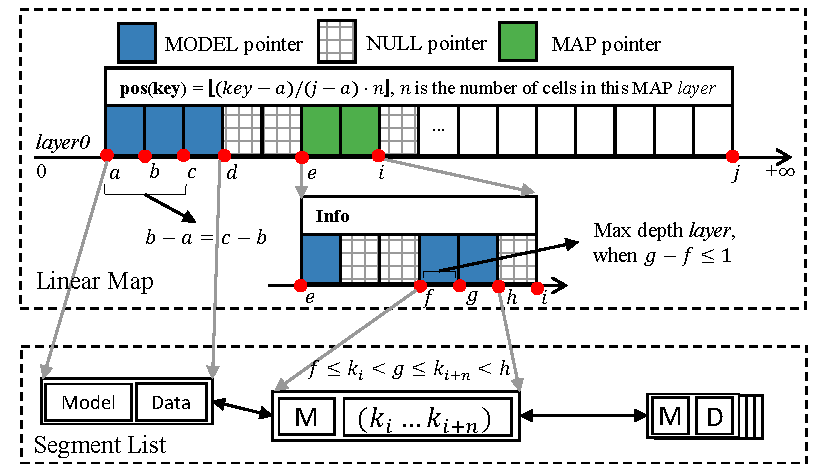
\includegraphics[width=1\linewidth]{main_structure.pdf}
    \caption{Main structure of LMIndex. Linear Map is its segment indexing structure. Each cell within a layer represents a fixed key interval, so the depth of the layer is maximized when the interval is $\le 1$. Precise routing to the covering cell is achieved through layer parameters, such as key range and cell count.}
    \label{fig:main-structure}
\end{figure}

% The main structure of LMIndex as depicted in Figure~\ref{fig:main-structure}, consists of a dual-layer architecture. The first layer, Linear Map, indexes specific segments, functionally analogous to the internal nodes of a B+Tree but with a flatter and more modifiable structure. The second layer, the segment list, comprises a collection of segments, each representing a single linear model and pointing to a data block, which is organized as an ordered linked list to support efficient range queries. To mitigate the performance impact of data updates, LMIndex incorporates additional structures. Specifically, we employ a memory-write optimized index skip list \cite{skiplist18} as a supplementary index.

LMIndex is an in-memory, space- and time-efficient versatile learned index paradigm designed to adapt to unknown or dynamic workloads and data
distributions. Its key idea is straightforward: use a lightweight yet effective structure that preserves high performance across diverse workloads without complex online tuning. To achieve this, LMIndex adopts a simple two layer architecture (Figure \ref{fig:main-structure}).

At the top layer, Linear Map (LM) efficiently identifies the target segment. As an auxiliary structure, LM neither requires online parameter tuning to maintain stability nor relies on costly model fitting. Instead, it structurally captures the key range distribution of the segments (i.e. $[key_{min}, key_{max}]$ for each segment). And it can locate the bottom segment in $O(1)$ time complexity when the key type is determined.

The bottom layer consists of an ordered sequence of segments, each primarily containing a linear model and the data layout. The linear model includes a range (max/min key), parameters, and an error threshold. To handle dynamic workloads, the segment implements a flexible update absorbing function, where incoming updates are first buffered locally by the segment. This buffering mechanism offers multiple architectural choices: it can employ an out-of-place structure, utilizing an additional secondary index like a red-black tree or a linked list, or an in-place structure, such as building child nodes similar to \cite{lipp21}. Within our framework, LMIndex employs a dense array coupled with an out-of-place buffer, whereas its variant, LMG, utilizes a gapped array as an in-place buffer. For LMG, we specifically employ an optimized gap allocation strategy. By distributing the reserved gaps more evenly across the array, this strategy reduces the average error search length and improves operational efficiency.

% For maximum space utilization, LMIndex stores data in compact arrays, while the variant LMG employs gapped arrays that trade some space efficiency for higher update absorption capacity.

% Although the architecture is simple, it proves remarkably effective because LM’s intrinsic properties complement the bottom layer’s efficiency. The top layer offers predictable, constant-time segment location, while the bottom layer’s optimized layout and model-based operations sustain high throughput and accuracy. Together, they enable LMIndex to achieve strong results across key metrics such as bulk loading, updates, queries, stability, and space usage.
% Due to the inherent quality of the structure, minimal modifications suffice to achieve substantial improvements.
% This design yields strong performance across six key metrics: bulk load, point query, range query, update, stability, and space usage.

This architecture is motivated by the goal of fully leveraging the inherent structural quality of the LM. Consequently, modest augmentations yield meaningful improvements, enabling the framework to strike a robust balance and secure advantages across multiple performance dimensions:

\textbf{Bulk load.} The bulk load consists of the construction of bottom layer and top layer. The bottom layer is constructed in $O(n)$ time by integrating a linear segmentation algorithm with the efficient model training algorithm, OETA. In the top layer, LM avoids complex approximation fitting, thus ensuring that the construction time overhead is $O(m)$ ($m$ is the number of segments, less than the data size). So the total complexity of bulk load is $O(n)$.

\textbf{Updates.} To handle dynamic workloads, the framework temporarily buffers incoming modifications locally within the segment before triggering a Structural Modification Operation (SMO) upon reaching a predefined capacity. At the bottom layer, this SMO functions similarly to localized bulk loading, retraining exclusively on the affected segment data to preserve error bounds. Meanwhile, at the top layer LM, the SMO incurs a theoretical $O(1)$ cost, adding only a marginal overhead to the overall update time.

\textbf{Stability.} Many learned indexes degrade after updates because structural changes disrupt query performance. LMIndex maintains stability by ensuring that the post-update structure resembles that of a freshly bulk-loaded index on the current data.

\textbf{Point and range queries.} Queries are decomposed into a top layer LM lookup and linear model prediction with error correction at the bottom layer. LM and OETA together ensure consistently low latency for both steps.

\textbf{Space usage.} Due to the optimal segmentation and compact structure, reducing space usage at the bottom layer is less effective. Thus, optimization focuses on the top layer LM, whose storage depends on the key range distribution of the segments. On real-world datasets, LM accounts for only about 4\% of the total index size in average. (see Section \ref{sec:lm_eval})

% Experiments on diverse datasets show that LMIndex matches or exceeds state-of-the-art learned indexes on most metrics and consistently outperforms B+Tree in both throughput and space efficiency, while requiring no workload-specific parameter tuning.

\subsection{Basic Operations}
\subsubsection{Point Queries and Range Queries}
For a point query with a search key $q$, the lookup process first traverses the top layer structure LM to locate the target segment, followed by a prediction and correction search within that segment. The LM is composed of flat pointer arrays (referred to as map layers), where each layer is composed of several cells. As illustrated in Figure \ref{fig:main-structure}, the key range of \textit{layer0} is $[a, j]$ and it contains $n$ cells. By simply computing $pos(key) = \lfloor (key - a)(j - a) \cdot n \rfloor$, one can precisely locate the corresponding cell for a given key. Each cell contains one of different types of Pointers: a MODEL pointer directs the query to the target segment; a NULL pointer terminates the search indicating the key is absent; and a MAP pointer advances the traversal to the next map layer. For a fixed key type, the routing complexity of LM is highly efficient and bounded by $O(1)$ since the maximum layer depth is finite (details in Section \ref{sec:lm}).

Within the targeted segment, LMIndex utilizes the linear model to predict the physical position of the query key $q$ within the data layout. If the initial prediction deviates from the exact location, a bounded binary search is executed within the segment's predefined error threshold. Upon locating a matching, non-deleted key, the corresponding record is returned. Otherwise, the query execution path falls back to probe the local buffering mechanism to resolve any recently inserted or modified records.

For range queries, they are initiated by locating the first key greater than or equal to the predefined lower bound, followed by a sequential scan that terminates upon exceeding the upper bound. As illustrated in Figure \ref{fig:main-structure}, contiguous segments are sequentially linked via bidirectional pointers, facilitating efficient cross-segment traversals while naturally bypassing invalidated or deleted keys. Notably, when a segment employs an out-of-place buffering mechanism, the framework dynamically merges keys residing in the primary data array with the ordered elements held in the secondary local buffer during this traversal. While this on-the-fly merging inevitably introduces a slight latency overhead, its theoretical time complexity remains $O(K)$ (where $K$ is the number of retrieved keys). Furthermore, to optimize execution during extensive range queries, the framework proactively probes the required capacity and pre-allocates contiguous memory prior to the scan, effectively eliminating the computational overhead of repeated dynamic resizing.

In detail, we explore the query mechanics of LM in Section \ref{sec:lm}. For the ``last-mile'' search within the segment, we demonstrate in Section \ref{sec:single-model} how binary search outperforms exponential search in complex distributions dataset, while OETA narrows the segment's error threshold so that binary search performs on par with exponential search under near-linear distributions.

% In Section \ref{sec:lm}, we explore the query mechanics of LM in greater detail. In Section \ref{sec:single-model}, we demonstrate how binary search outperforms exponential search in complex distributions dataset and show that OETA optimizes binary search to match the performance of exponential search under ideal linear distributions.

\subsubsection{Update}
\label{sec:update}
The insertion process initiates by routing the new key to its target segment. If the corresponding physical slot is occupied by a logically deleted record, the new key is directly inserted in-place. Conversely, the framework delegates the insertion to the segment's local buffering mechanism. To preserve the efficiency of the sequential scans, this local buffer maintains all newly absorbed elements in an ordered state. The maximum capacity of this buffer serves as a configurable parameter. Once the predefined capacity is saturated, the segment merges the buffered records and triggers a local Structure Modification Operation (SMO) to retrain the model.

% Rather than using least-squares retraining, LMIndex apply an optimal segmentation retraining method, which may produce additional segments but is more efficient and better integrated with OETA. Retraining may produce residual segment (containing than $2\varepsilon$ keys) and it only appears at the end of list. To avoid its negative impact on lookup efficiency, we first attempt to merge the residual keys into the next segment, provided the resulting error remains within the $\varepsilon$-constraint. If the merge fails, they are jointly retrained. This residual-handling strategy may trigger chain updating, but this guarantees optimal segmentation, ensuring stability even in heavy write workloads. Further optimizations for this issue are presented in LMG (Section \ref{sec:lmg}).

For retraining, LMIndex employs OETA to train segment parameters. While it shares the same Big-O complexity as Least Squares (LS), its computational overhead is typically significantly lower in practice (see Section \ref{sec:oeta}). Prior to training, we apply the segmentation algorithm from \cite{pgm20} to partition the data. This process may yield a residual segment at the tail containing fewer than $2\varepsilon$ ($\varepsilon$ is the global error threshold) keys. To avoid its negative impact on lookup efficiency, we first attempt to merge the residual keys into the next segment, provided the resulting error remains within the $\varepsilon$-constraint. If the merge fails, they are jointly retrained. This residual-handling strategy may trigger cascading retraining, but this guarantees optimal segmentation, ensuring stability even in heavy write workloads. Further optimizations for this issue are presented in LMG (Section \ref{sec:lmg}).

% In addition, when an insertion modify the maximum key of a segment, LM updates LM to maintain the correctness of segment index.
% The retrained segment list may contain tail residuals, small segments (contain less than $2\varepsilon$ keys) that only appear at the end of list. To minimize the impact of these small segments on LM performance, we first attempt to insert the residual data into the preceding segment (if it does not exceed the $\varepsilon$-constraint). If this is not possible, the segment and its successor undergo retraining. Handling residuals may lead to chain updates, but this guarantees optimal segmentation, ensuring stability even in heavy-update scenarios. Further optimizations for this issue are presented in LMG (Section \ref{sec:lmg}). Insertion can also result in a change to a segment’s maximum value, requiring adjustments to the LM structure.

For deletions, if a matching key is found within a segment, LMIndex marks the key with a tombstone. In-place deletion ensures that deletion efficiency is generally similar to querying. To maintain stability, LMIndex reallocates data after deletion: when the number of valid keys within a segment falls below global $\varepsilon$, the largest key from the preceding segment is moved and placed in front of the segment. If this insertion does not satisfy the $\varepsilon$-constraint, or if the number of valid keys in the previous segment is less than $\varepsilon$ + 1, the current and the previous segment are merged and retrained.

% Whenever a segment’s range changes, due to insertion or deletion, adjustments to the LM must be made to maintain the correctness of segment index. This process is highly efficient and contributes only a negligible overhead during retraining. Further details of LM updates are covered in Section \ref{sec:lm}.

When insertions or deletions shift a segment’s key range, LM is updated to maintain segment routing. Because these changes are confined to affected segment boundaries, the update cost is negligible compared to retraining. Section~\ref{sec:lm} elaborates on LM’s update handling in detail.

\subsubsection{Bulk Load}
% LMIndex supports efficient bulk load operations without relying on heuristic cost models or complex segmentation procedures. Instead, it uses a data-aware segmentation algorithm that partitions the sorted input using a global error threshold, implicitly adapting to local distribution complexity and generating more segments in non-linear locality.

Bulk load consists of splitting the data, training the model, and building the segment index. First, LMIndex splits data using the algorithm in \cite{pgm20}. Given a global error threshold $\varepsilon$, it ensures each segment admits at least one linear function fitting all points within error bound $\varepsilon$.

% Unlike some learned indexes, which rely on cost models or segmentation models, LMIndex leverages a data-aware algorithm to maintain high efficiency and performance during the build process. Specifically, we use a segmentation algorithm based on a given global error threshold to partition the data, implicitly fitting the data distribution and creating more segments in complex local distributions.

Secondly, to further improve local accuracy, we introduce OETA, which efficiently computes the minimum error threshold and corresponding model parameters for each segment. OETA enhances local adaptivity of models, enabling smaller correction ranges. For instance, if global $\varepsilon = 64$ but the optimal threshold for a segment is $2$, correcting within that segment requires only $\log_2(2) = 1$ steps, i.e., a $\log_2(64)/\log_2(2) = 6\times$ reduction in correction steps when using binary search.

% OETA allows deeper fitting of the data distribution within each segment range. For example, if the initial error threshold is $\varepsilon = 64$, and the minimum error threshold of a segment is $2$, OETA combined with binary search offers a theoretical performance improvement of $log(64)/log(2) = 6$ times.

% At the top layer of LMIndex, we designed an LM structure that eliminates the need for complex model fitting. The construction cost depends on the number of segments $m$ and their local distribution, with a theoretical complexity of $O(m)$. The LM structure exhibits characteristics of both tree-like and flat architectures, allowing it to sense the distribution of models. When a model’s range is large, it resides in a shallower map layer; when the range is smaller, it moves to a deeper map layer. We will discuss the LM construction details in Section \ref{sec:lm}.

Finally, segments are indexed by the LM structure. LM is a shallow, hierarchical structure with theoretical construction cost $O(m)$, where $m$ is the number of segments. Larger range segments are placed in higher layers with coarser granularity, while smaller ranges descend into finer levels, allowing LM to adapt to segment range distribution. Detailed LM construction procedures are discussed in Section~\ref{sec:lm}. Total complexity of bulk loading is $O(n)$.

\subsection{LMIndex with Gaps (LMG)}
\label{sec:lmg}
LMG is a variant of LMIndex tailored to raise update throughput while preserving query efficiency. The primary structural modification in LMG is it replaces compact array with gapped array. And we introduce an expansion rate $\tau$ to control the additional space allocated for gaps.

Allocating gaps in a gapped array is usually implemented by inserting keys. Standard model-based insertion \cite{alex20} places a new key at its predicted position $f(k)$ or the nearest available empty slot. However, this approach accumulates localized errors under data skew. Formally, we define a contiguous sequence of inserted keys $K = \langle k_1, \dots, k_s \rangle$ as a \textit{many-to-one} subset if the prediction model maps them to the exact same position, i.e., $\forall k_j \in K, f(k_j) = C$, where $s = |K|$. Sequential insertion of $K$ forces the final key $k_s$ to position $C + s - 1$, yielding a lower-bound maximum error of $s-1$.

To mitigate this effect, LMG introduces a reserved-space insertion strategy that calculates an optimized starting physical index $P_{start}$ for the first key $k_1$. The allocation is strictly constrained by two spatial boundaries. Let $pos(x)$ denote the allocated physical index of key $x$. The lower bound $C_f$ is defined as $C_f = \max_{k'<k_1} (pos(k')) + 1$. Symmetrically, the upper bound $C_b$ is defined as $C_b = \min(f(k_{s+1}), N)$, where $N$ is the array capacity.

Given the predicted position $C$, subset size $s$, segment error threshold $\varepsilon_i$, and the spatial bounds $[C_f, C_b]$, the strategy dynamically determines $P_{start}$ through the following piecewise function:
$$ P_{start} = \begin{cases}
C_f & \text{if } C - C_f \le s/2 \\
\max(C_f, C - \varepsilon_i, C_b - s) & \text{if } C_b - C \le s/2 \\
C - s/2 & \text{otherwise}
\end{cases} $$
Following $k_1$, the remaining keys $k_j \in K$ ($2 \le j \le s$) are inserted contiguously at physical indices $pos(k_j) = P_{start} + j - 1$.

Functionally, this formal allocation aligns dense many-to-one subsets symmetrically to minimize localized maximum errors, while maintaining the same behavior as model-based insertion for other keys.

% Allocating gaps in a gapped array is usually implemented by inserting keys. The model-based insertion \cite{alex20} places the key at the predicted position if it's empty, or at the nearest empty position thereafter. However, it would suffer a larger maximum error for many-to-one subsets:

% A contiguous subset of keys $K = \{k_1, k_2, \dots, k_s\}$ is many-to-one subset if $\forall k \in K, f(k) = C$, where $f(x)$ is prediction model and $s = |K|$. Model-based insertion yields the least $s - 1$ maximum error when many-to-one subset are encountered.

% To mitigate the many-to-one subset effect, LMG proposes a reserved-space insertion strategy. It records the current minimum insertable position $C_f$ and an upper bound $C_b = \min(f(k_{s+1}, N)$ ($N$ is the gapped array size). The strategy operates as follows: (1) If $C - C_f \le s/2$, the first key $k_1$ is placed at $C_f$; (2) If $C_b - C \le s/2$, $k_1$ is placed at $\max(C_f, C - \varepsilon_i, C_b-s)$; (3) Otherwise, $k_1$ is placed at $C - s/2$. Other keys in $K$ are inserted contiguously after $k_1$. Functionally, this strategy adapts the insertion to reduce the prediction error for many-to-one subsets, while maintaining the same behavior as model-based insertion for other keys.

For updates, LMG employs a gapped array as its in-place buffering mechanism. While this in-place design introduces additional space overhead compared to out-of-place alternatives, it removes the overhead associated with cross-structure data access and on-the-fly merging during queries. During an insertion, the framework identifies the target slot and shifts the nearest available gap to accommodate the new key. To bound insertion latency, gap movement is restricted to a constant multiple of $\varepsilon$ (e.g., $8\varepsilon$). Furthermore, to prevent the cascading retraining issue discussed in Section \ref{sec:update}, LMG merges any residual tail segment shorter than $2\varepsilon$ into the preceding segment. Although this method slightly relaxes the $\varepsilon$-constraint, it effectively avoids cascading retraining overhead and segment fragmentation.

To guarantee semantic correctness of search despite potential update, LMG adopts a binary–then–exponential hybrid search strategy. It first performs a binary search bounded by the segment's error threshold, and falling back to exponential search if the target position is not located. As show in Section \ref{sec:choose-correction}, this design prioritizes binary search because it's more effective on complex data distributions.

\section{Linear Map}
\label{sec:lm}
In learned indexes based on piecewise linear models, the major overhead of queries typically stems from locating the correct segment and performing last-mile correction within it. Linear Map (LM) focuses on segment localization, achieving theoretical $O(1)$ query and update complexity. Its space complexity is $O(m)$, where $m$ is the number of segments, and the actual memory footprint adapts to the distribution of segment ranges.
\begin{figure}[h]
    \centering
    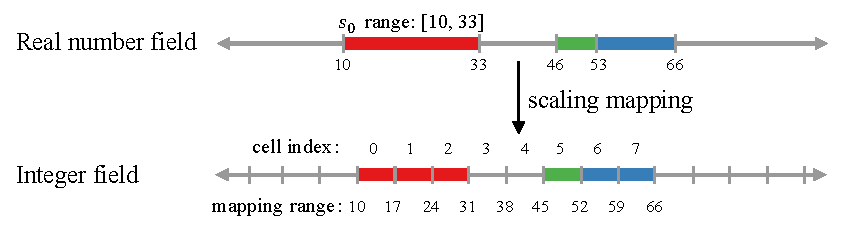
\includegraphics[width=\linewidth]{lm_mapping.pdf}
    \caption{Key idea of LM: Mapping segment range from the real number field to the integer field, ensuring each segment corresponds to at least one integer cell.}
    \label{fig:lm-mapping}
\end{figure}

\subsection{Single-layer LM}
\label{sec:sl-lm}
Let $S = \{s_1, s_2, \dots, s_m\}$ denote an ordered set of non-overlapping segments, where each segment $s_i$ corresponds to the range of keys $[min_i,max_i]$ with width $R(s_i) = max_i - min_i$. These segments can be naturally viewed as intervals over the real number field, as illustrated in Figure \ref{fig:lm-mapping}.

To enable direct lookup without probing, Linear Map projects the continuous key range onto a flat indexable array, referred to as the \textit{layer}. Each cell in the \textit{layer} represents a fixed-length subrange of the key domain and stores either a pointer MODEL to the segment that covers that subrange or NULL if no segment overlaps it.

To ensure that every segment occupies at least one cell, LM guarantees minimum resolution over the key range $[min_1, max_m]$. Let $R(layer) = max_m - min_1$ and $|layer|$ be the number of cells in layer, the minimum resolution is:
$$
\min |layer| = \left\lceil R(layer) / \min R(s_i) \right\rceil
$$

LM adopts this minimal resolution to optimize space usage. Under this resolution, LM applies a scaling mapping formula (SMF) to directly compute the cell index for a key:
$$
\text{SMF}(key) = \left\lfloor (key - min_1) / R(layer) \cdot |layer| \right\rfloor
$$

We next show that SMF guarantees that the endpoints of every segment map to different cells when $|layer|$ equals the minimum required resolution. Let $d = \min R(s_i)$, and consider a segment range $[k_a, k_a + d]$. Then:
% &\text{SMF}(k_a + d) = \left\lfloor (k_a + d - min_1) / R(layer) \cdot \left\lceil R(layer) / d \right\rceil \right\rfloor \\
% &\geq \left\lfloor (k_a - min_1) / R(layer) \cdot \left\lceil R(layer) / d \right\rceil  + 1\right\rfloor = \text{SMF}(k_a) + 1
$$
\begin{aligned}
&\text{SMF}(k_a + d) \geq \left\lfloor (k_a - min_1) / R(layer) \cdot \left\lceil R(layer) / d \right\rceil\right\rfloor + 1 \\
&\text{SMF}(k_a + d) \le \left\lfloor (k_a - min_1) / R(layer) \cdot \left\lceil R(layer) / d \right\rceil \right\rfloor + 2
\end{aligned}
$$

Since $\text{SMF}(k_a) = \left\lfloor (k_a - min_1) / R(layer) \cdot \left\lceil R(layer) / d \right\rceil\right\rfloor$, $\text{SMF}$ $(k_a + d)$ is bounded by $[\text{SMF}(k_a) + 1, \text{SMF}(k_a) + 2]$, ensuring that each segment occupies at least one distinct layer cell and preventing boundary collapse.

Importantly, SMF is used for both queries and updates. Although it is a linear function, it differs from linear predictive models in that it requires no training. All parameters are derived directly from the known properties of the segment set $S$, enabling it to dynamically adapt to changes in the segment layout.

To construct a single-layer LM, the \textit{layer} is first initialized with NULL pointers. For each segment $s_i$, its range $[min_i,max_i]$ is projected to the cell range $[\text{SMF}(min_i), \text{SMF}(max_i)]$, and each cell in this range is filled with a MODEL pointer link to $s_i$. When adjacent segments $s_j$ and $s_{j+1}$ share a boundary cell, i.e., $\text{SMF}(max_j) = \text{SMF}(min_{j+1})$, LM assigns this cell to $s_{j+1}$. This minimum-first boundary rule consistently resolves ties without ambiguity and preserves correctness.

For point queries, SMF computes the target cell in $O(1)$ time. Every key is deterministically mapped to its corresponding cell with perfect accuracy. In most cases, the cell contains the correct segment pointer. In boundary cases where a key near the tail of segment $s_j$ falls into the first cell of $s_{j+1}$, LM performs a single fallback step to $s_j$ via the segment list, ensuring correctness with constant overhead.

For updates, LM locates the affected cells via SMF and replaces them with NULL or new MODEL pointers. The update cost is proportional to the number of cells traversed.

\subsection{Multi-layer LM}
\label{sec:ml-lm}
The single-layer LM represents an conceptually unbounded flat array, with space complexity $O(\min |layer|)$. Since the theoretical lower bound for indexing $m$ segments is $O(m)$, the single-layer LM amplifies:
$$
O(\min |layer|/m) = O\left( (R(layer)/m) / \min R(s_i) \right)
$$

When the distributions is skewed or non-linear, $\min R(s_i)$ may be orders of magnitude smaller than the average segment width $R(layer)/m$, resulting in excessive space usage, poorer cache locality, and higher average update cost. Moreover, future insertions that further reduce $\min R(s_i)$ force a full rebuild of the single-layer LM, incurring considerable overhead.

To avoid these limitations, we introduce the multi-layer LM, which bounds each \textit{layer} size by a constant $\mathit{L}$. As shown in Figure \ref{fig:main-structure}, it combines flat and tree-like designs: each \textit{layer} maps a flat key interval and each cell may store a MAP pointer to another \textit{layer}, recursively refining the mapping.

Each \textit{layer} covers a key range $[min_{layer}, max_{layer}]$ and indexes a contiguous subset of segments $S' = \{s_j, ..., s_{j+t}\}$ with $min_j \ge min_{layer}$ and $max_{j+t} \le max_{layer}$. Its minimum resolution is:
$$
\min|layer| = \left\lceil R(layer) /\min R(s_{i'}) \right\rceil, \quad i' \in [j, j+t]
$$

and the associated SMF becomes:
$$
\text{SMF}(key) = \left\lfloor (key - min_{layer}) / R(layer) \cdot |layer| \right\rfloor
$$

\begin{algorithm}[h]
  \caption{BuildMultiLayerLM}
  \label{alg:build-mlLM}
  \small 
  \KwIn{$S$: the set of segments, $\mathit{L}$: max layer size}
  \KwOut{$lm$: Multi-layer LM}
  $k_0 \gets$ left range bound of $S$\;
  descending sort $S$ by $R(s)$, $s \in S$\;
  $s' \gets$ pop($S$)\;
  $min\_size \gets \lceil R(S) / R(s') \rceil$\;
  $lm \gets$ an array of size $\min(\mathit{L}, min\_size)$\;
  $rate \gets$ size($lm$) $/ R(S)$\;
  \While{$min\_size > \mathit{L}$ and $S$ is not empty}{
    $pos_1 \gets $ int($(min_{s'} - k_0) \times rate$);\tcp{\small Scaling mapping}
    $pos_2 \gets $ int($(max_{s'} - k_0) \times rate$)\;
    \If{$pos_1 = pos_2$ and $lm[pos_1] = NULL$}{
    \tcp{\small Build a child layer}
        $S' \gets \{s'\}$\;
        range($S'$) $\gets$ mapping\_index($lm[pos_1, pos_2]$)\;
        $lm[pos_1] \gets $BuildMultiLayerLM($S'$, $\mathit{L}$)\;
    }
    \Else {
        draw\_multi\_layer\_map($lm$, $pos_1$, $pos_2$, $s'$)\;
    }
    $s' \gets$ pop($S$)\;
    $min\_size \gets \lceil R(S) / R(s') \rceil$\;
  }
  $S \gets S \cup s'$\;
  \tcp{\small Draw remaining segments, they don't build new layers}
  \For{$s \in S$}{
    $pos_1 \gets $ int($(min_{s} - k_0) \times rate$)\;
    $pos_2 \gets $ int($(max_{s} - k_0) \times rate$)\;
    draw\_multi\_layer\_map($lm$, $pos_1$, $pos_2$, $s$)\;
  }
  \Return{$lm$;}
\end{algorithm}

Algorithm \ref{alg:build-mlLM} summarizes the recursive construction of the multi-layer LM. In lines 4 and 17, we compute the minimal resolution for the current segment. If it exceeds $\mathit{L}$ and this segment collapses into one cell, we recurse (lines 11–13) to build a child \textit{layer}. Recursion continues until the mapped range spans at least two distinct cells. The helper function \textit{draw\_multi\_layer\_map()} fills the mapped cells and ensures correct pointer assignment at segment boundaries.

Each child layer can refine current resolution by a factor of $\mathit{L}$, while occupying only one cell in its parent \textit{layer}, yielding a compact but arbitrarily fine-grained hierarchical mapping.

\textbf{Queries.} Querying follows the same SMF-based mapping strategy. Given a key, multi-layer LM computes its target cell via SMF. If the cell contains a MAP pointer, the query proceeds recursively to the next \textit{layer}. This process repeats until the result points to a MODEL or a NULL. Although hierarchical, the maximum layer depth is bounded by a small constant (see Section~\ref{sec:ca-lm}), ensuring an overall query cost of $O(1)$, making multi-layer LM suitable for high-performance lookup workloads.

% \textbf{Insertions.} If a segment $s_i$ maps to a single cell (i.e., $\text{SMF}(min_i) = \text{SMF}(max_i)$) and the target cell is not a MAP, LM checks whether the required resolution exceeds $\mathit{L}$. If not, the current layer is scaled; otherwise, a lower \textit{layer} is constructed recursively until the segment spans multiple cells. In most cases, segments span multiple cells (i.e., $\text{SMF}(min_i) \ne \text{SMF}(max_i)$), requiring only direct assignment of MODEL or NULL pointers to the computed cell range. At the root level, if insertions extend the overall key range and the \textit{layer} size exceeds $2\mathit{L}$, we trigger a rebuild to maintain a compact layout.

\textbf{Insertions.} Insertions also follow SMF-based localization. (1) If a segment spans multiple cells ($\text{SMF}(min_i) \ne \text{SMF}(max_i)$), pointers are directly written to the mapped range. (2) If a segment maps to a single cell and the cell is not a MAP, LM checks whether the required resolution exceeds $\mathit{L}$. If so, it recursively constructs a child layer; otherwise, it scales the current layer by an integer multiple. (3) At the root level, when insertions extend the global key range and the layer size exceeds $2\mathit{L}$, LM triggers a rebuild to maintain compact layout.

\textbf{Deletion.} Since the query computation is independent of \textit{layer} size, LM does not shrink the \textit{layer} even when $\min R(s_{i'})$ increases due to deletions. A non-root \textit{layer} is only removed when its segment subset $S'$ becomes empty. At the root, if the total key range shrinks such that the ideal resolution falls below 25\% of the current layer size, LM triggers a rebuild to restore efficient memory utilization and stable query performance.

\subsection{Complexity Analysis of LM}
\label{sec:ca-lm}
In practice, LMIndex employs a multi-layer Linear Map. Unless otherwise noted, the following analysis assumes a multi-layer LM by default.

\subsubsection{Query Complexity}
\label{sec:lm-query-complexity}
% Within each layer, a query requires only constant-time computation using the SMF. Thus, the overall query complexity is $O(t)$, where $t$ is the maximum depth of multi-layer LM. Because each layer expands the address space by up to $\mathit{L}$ times, for any constant $a \ge 1$, choosing $\mathit{L}$ such that $\mathit{L}^a > 2^b$ for a $b$-bit key domain guarantees $t \le a$ and hence $O(t)=O(1)$. For example, setting $\mathit{L} = 65536$ (i.e., $2^{16}$) allows for up to $\mathit{L}^5 \approx 1.2 \times 10^{24}$ MODEL cells, which far exceeds the $2^{64} \approx 1.8 \times 10^{19}$ unique values of a 64-bit key. Even in the extreme case where each segment holds only a single key, this hierarchical capacity remains sufficient.

% Furthermore, following \cite{pgm20}, each segment must contain at least $2\varepsilon$ keys, which increases the minimum segment range. Empirical results (see Table \ref{tab:lm_info}) further confirm that the actual depth $t$ remains small in practice.

Within each layer, a query requires only constant-time computation using the SMF. Thus, the overall query complexity is $O(t)$, where $t$ is the maximum depth of multi-layer LM. Let $\mathit{L} = 2^l$, then the depth $t$ is given by $t = \log_\mathit{L}(\mathtt{R}) = \log_2(\mathtt{R}) / l$, where $\mathtt{R} = R(S)/\min R(s_i)$. Since the key type determines a fixed bit-width $b$, $\mathtt{R}$ is naturally bounded by $m \le \mathtt{R} \le 2^b$, where $m$ is the number of segments. Note that $\mathtt{R}$ decreases as the distribution becomes more linear or as the segment ranges become more uniform. Consequently, $O(t) = O(b/l) = O(1)$, since both $b$ and $l$ are constants.

Following this logic, in theoretically, any $O(\log n)$ index is also $O(1)$ because $n \le 2^b$. However, in practice, significant distinctions exist between the LM and such traditional structures (e.g., B+Tree): First, thanks to the $O(1)$ intra-layer search cost enabled by the SMF, $l$ can be configured to be sufficiently large, thereby effectively reducing the theoretical upper bound of $t$. In contrast, B+Trees employ binary search within each node, which constrains the node size (fan-out) to maintain efficiency. Second, the depth of the LM is independent of the dataset size, whereas the depth of a B+Tree scales strictly with that size. Notably, when $n$ approaches $2^b$, the data becomes highly linear, causing the LM depth to converge to its minimum. Finally, the above derivation assumes each segment contains only a single key. In reality, \cite{pgm20} proves each segment contains at least $2\varepsilon$ keys, resulting in a smaller depth.

For instance, with $\mathit{L} = 65536$ (i.e., $2^{16}$) and standard 64-bit keys, the depth is bounded by $t \le 64 / 16 = 4$. Empirical results (see Table \ref{tab:lm_info}) further confirm that the actual depth $t$ remains small in practice.

While increasing $\mathit{L}$ reduces $t$, excessive values yield diminishing returns. Larger values of $\mathit{L}$ may increase space consumption, harm cache locality, and degrade update efficiency. Importantly, $\mathit{L}$ serves as an adaptive upper bound rather than a fixed capacity, allowing LM to adjust layer sizes dynamically according to segment distribution. In practice, setting $\mathit{L} = 65536$ achieves a favorable balance between query efficiency and space overhead.

\subsubsection{Update Complexity}

In the single-layer LM, the cost of updating a segment $s_i$ is determined by the number of cells it occupies:
$$
\text{SMF}(max_i) - \text{SMF}(min_i) \le R(s_i) / R(layer) \cdot |layer| + 1
$$

% If the layer size $|layer|$ is set to the minimum resolution, each segment occupies at least one cell. The $\min R(s_i)$ segment occupies a constant number of cells, thus its update complexity is $O\left(\min R(s_i) / R(layer) \cdot |layer|\right) = O(1)$. For a general segment $s_i$, the update cost grows proportionally to its width relative to the smallest segment, i.e., $O(R(s_i) / \min R(s_i))$.

For a segment with the minimum key range length $\min R(s_i)$, the number of occupied cells is constant. Thus, the update cost is $O\left(\min R(s_i) / R(layer) \cdot |layer|\right) = O(1)$. Consequently, the update cost for a general segment $s_i$ is quantified as $O(R(s_i) / \min R(s_i))$.

Considering amortized complexity across $m$ segments, we obtain:
$$
O\left(\frac{1}{m} \sum_{i=1}^{m} R(s_i) / \min R(s_i) \right) = O\left(\text{avg}(R(s_i))/\min R(s_i)\right)
$$

Hence, the more the width of the segment tends to be uniform ($\text{avg}(R(s_i))\xrightarrow{}\min R(s_i)$), the closer the amortized cost is to $O(1)$.

% In the multi-layer LM, updating a segment requires first locating the target \textit{layer} in $O(t)$ time. Within that layer, updates affect at most $O(\mathit{L})$ cells, following the same logic as the single-layer case. Since segment boundaries may span multiple layers, updates may involve up to $O(t\mathit{L})$ cells. Additionally, update operations may create or delete child layers, with cost denoted as $u$. Based on Section \ref{sec:lm-query-complexity}, and setting $\mathit{L}$ large enough depending on the key type, we get:
% $$
% O(t + \mathit{L} + t\mathit{L}) + u = O(t\mathit{L}) + u = u
% $$

% Here, $u \le O(t\mathit{L})$ since at most $O(t\mathit{L})$ space is allocated or released per update. So the update cost of multi-layer LM is $O(1)$. In practice, layer creation is rare and most updates modify only a few cells; lazy reclamation further amortizes cleanup overhead.

In the multi-layer LM, updating a segment requires first locating the target \textit{layer} in $O(t)$ time. Within that layer, updates affect at most $O(\mathit{L})$ cells, following the same logic as the single-layer case. Since segment boundaries may span multiple layers, updates may involve up to $O(t\mathit{L})$ cells. Based on Section \ref{sec:lm-query-complexity}, and setting $\mathit{L}$ large enough depending on the key type, we get:
$$
O(t + \mathit{L} + t\mathit{L}) = O(t\mathit{L}) = O(1)
$$

% Here, $u \le O(t\mathit{L})$ since at most $O(t\mathit{L})$ space is allocated or released per update. So the update cost of multi-layer LM is $O(1)$. 

Layer allocation or release is triggered when the current layer fails to assign at least one cell to a new segment, or when the deletion of an existing segment renders the layer empty. While this process may cascade, it affects at most $t\mathit{L}$ cells. In practice, most updates modify only a few cells. Layer allocation is infrequent, while lazy reclamation further amortizes the overhead of release.

LM's rebuilds are only triggered when the root layer becomes highly unbalanced, e.g., if the size of the root layer is exceeds $2\mathit{L}$ or the theoretical resolution is 25\% of the current size. Since each rebuild exponentially adjusts $R(layer)$, the probability of repeated rebuilds rapidly decreases.

Notably, LM does not require rebuilding to maintain correctness. It maintains robust query and update performance under distribution shifts, tolerating accumulated updates via bounded space redundancy rather than accuracy loss. Stability experiments in Section~\ref{sec:stability} confirm this resilience.

% Its query and update performance is robust under data distribution shifts, especially when the whole key range remains stable. In contrast to other learned indexes, LM tolerates accumulated updates by introducing space redundancy, not accuracy degradation. Stability experiments \ref{sec:stability} further validate this robustness.

\subsubsection{Space and Construction Complexity}

In multi-layer LM, each segment occupies at most $O(t\mathit{L}) = O(1)$ space under a fixed key type. Given that there are $m$ segments in total, the overall space complexity of LM is $O(mt\mathit{L}) = O(m)$. In fact, $O(t\mathit{L})$ is quite loose. Table~\ref{tab:lm_info} demonstrates that the average number of cells per segment is far smaller than the theoretical peak value $t\mathit{L}$. Additionally, since LM requires no model retraining, its construction overhead primarily consists of pointer allocation. Consequently, the construction complexity aligns with the space complexity, both being $O(m)$.

To understand how space grows with $\mathit{L}$, we consider the worst-case bound $t\mathit{L} = \mathit{L} \cdot \log_\mathit{L}\mathtt{R}$.

Where $\mathtt{R} = R(S) / \min R(s_{i})$ is regarded as a constant related to the dataset, we compute the derivative:
$$
\frac{d}{d\mathit{L}} \left(\mathit{L} \cdot \log_\mathit{L} \mathtt{R}\right) = \ln \mathtt{R} \cdot \frac{\ln \mathit{L} - 1}{(\ln \mathit{L})^2}
$$

So when $\ln \mathtt{R} > 0$, this function achieves its minimum at $\mathit{L} = 3$ ($\mathit{L}$ is an integer), representing the theoretical space-optimal max layer size. For $\mathit{L} > 3$, the function increases monotonically. 

% However, this bound is loose. In practice, as shown in Table \ref{tab:lm_info}, the average segment cell is significantly smaller than $O(t\mathit{L})$. Due to LM’s adaptive layer allocation, larger values of $\mathit{L}$ may reduce space overhead. For instance, consider $9$ adjacent segments of equal range: when $\mathit{L} = 3$, they require $12$ cells, while setting $\mathit{L} \ge 9$ reduces the requirement to $9$ cells.

In practice, space usage is closely tied to the model distribution. Due to LM’s adaptive layer allocation, larger values of $\mathit{L}$ can sometimes reduce space overhead. For instance, consider $9$ adjacent segments of equal range: when $\mathit{L} = 3$, they require $12$ cells, while setting $\mathit{L} \ge 9$ reduces the requirement to $9$ cells.


% \textit{Linear Map} (LM) is a structure designed for indexing segments of PLM, featuring low construction cost and optimal query cost, while its variant also achieves theoretical optimality in updates. LM's space usage depends on the data distribution, and experiment \ref{sec:lm-evaluation} demonstrate its efficiency due to the minimized array design.

% \subsubsection{General LM}
% \label{sec:glm}
% General LM employs a flat structure for indexing segments, deviating from most updatable learned indexes that utilize tree structures \cite{lipp21, madex20, fiting-tree19}. This flat design inherently reduces the routing path length, lowering the routing complexity from $O(log)$ to $O(1)$ overhead. State-of-the-art learned index SWIX\cite{swix24} also adopts a flat structure, demonstrating its efficiency compared to tree-based structures. However, unlike SWIX, LM's construction requires no model training, granting it advantages in bulk-loading and updates, particularly in high-frequency update scenarios. By benefiting from lower construction costs (Section \ref{sec:lm-evaluation}), LM can serve as a general PLM segment indexing structure. This allows developers to focus primarily on the model itself. Furthermore, LM's decoupling from specific models enables its adaptation to various piecewise models, including non-linear ones, making it a versatile and valuable tool in diverse indexing scenarios.

% LM is a structure that maps the real number field to an integer \emph{array}. Given a segment set $S = \{s_0, s_1, ... , s_{m-1}\}$, where $s_i \in S$ and is ordered within $S$, the data range of $s_i$ is denoted as $[min_{s_i}, max_{s_i}]$. As illustrated in Figure~\ref{fig:lm-mapping}, we can draw the real number map of $S$ on a number line, with a range of $[min_{s_0}, max_{s_{m-1}}]$, and each $s_i$ is represented by a line segment $[min_{s_i}, max_{s_i}]$. The range length of $s_i$ is denoted as $R(s_i) = max_{s_i} - min_{s_i}$, and similarly for $R(S)$. LM scales the real number map to an integer array, where each integer represents an equal-length range in the real number field and also corresponds to a cell in the array. Pointers to the segments $s_i$ are placed in these cells, ensuring that each $s_i$ exists in at least one cell. To achieve this, the array size is increased to improve the resolution of the integer map, making the mapping range length of integers smaller than $\min (R(s_i))$. To maintain space efficiency, LM uses the minimum array size that satisfies this requirement: 
% \begin{equation}
% \label{eq:min-layer-size}
%   \min (R(array)) = \lceil R(S) / \min (R(s_i))\rceil
% \end{equation}

% Each segment in LM has at least one mapping cell. The range of $s$ in the array are defined by the scaled mapping of $min_s$ and $max_s$. The scaled mapping is also used for querying:
% \begin{equation}
% \label{eq:cal-pos}
%   pos(key) = \lfloor (key - min_{s_0}) / R(S) \times R(array)\rfloor
% \end{equation}

% All parameters are derived from prior knowledge, making the scaled mapping calculation $O(1)$ in complexity. LM updates also employ a similar approach, which is discussed in detail in Section \ref{sec:lm-update}, along with complexity analysis.

% \subsubsection{Multi-layer LM}
% Indexing $m$ segments takes at least $O(m)$ space. According to the formula \eqref{eq:min-layer-size}, the size of LM is not determined by $m$ but by the ratio of the $S$ length to the minimum segment length. Due to the potential empty gaps in $S$, $\sum R(s_i)\le R(S)$. Consequently, $\min(R(s_i)) \le R(S) / m$, and $\min (R(array)) = R(S) / \min(R(s_i)) \ge m$. Furthermore, the relationship between $\min(R(array))$ and $m$ is as follows:
% \begin{equation*}
%   \min (R(array)) / m =(R(S) / m) / \min(R(s_i))
% \end{equation*}

% The ratio $R(S) / m$ is referred to as the magnification factor. Intuitively, the larger the ratio of the dense average segment length $R(S) / m$ to $\min(R(s_i))$, the more space LM occupies compared to $O(m)$. Table \ref{tab:lm-stat} presents the magnification factor observed in real-world datasets. This magnification can lead to substantial space overhead when the data is highly skewed. To address this issue, we propose the Multi-layer LM, a variant that introduces an additional parameter and slightly compromises query performance. Unless otherwise specified, LM refers to Multi-layer LM in the subsequent sections.

% Multi-layer LM introduces the concept of layers, with a maximum size $\mathit{L}$ for each layer, which also represents the maximum resolution for each layer. The construction of the Multi-layer LM outlined in Algorithm \ref{alg:build-mlLM}. If $s'$ is defined as the minimum length segment such and its $\min (R(array))$ exceeds $\mathit{L}$, then the mapping range of $s'$ cannot cover a single cell. To represent $s'$, we expand the cell containing $s'$ to form a new layer. In the subsequent layer, with a reduced data range, the resolution can increase by up to $\mathit{L}$ times compared to the previous layer. The algorithm iteratively checks if $\min (R(array))$ for $s'$ exceeds $\mathit{L}$, and if so, it continues building the next layer until a layer is found where the segment can be represented by at least one cell.

% In contrast to a B+Tree, the query in the Multi-layer LM is independent of $\mathit{L}$, allowing us to set $\mathit{L}$ to a significantly large value. We set $\mathit{L} = 65536$ in our experiments, which enables each layer to contain more information while maintaining a low layer height. In our approach, we calculate the mapping position using formula \eqref{eq:cal-pos}, requiring only one calculation per layer to find the exact position. Despite the multi-layer structure, our queries remain efficient, as the resolution grows exponentially with layer height, allowing for an exponential increase in the number of representable segments. In our setup, even with a layer height of only 5, we can index a segment set with $\min (R(array))>10^{24}$. We will discuss the details of querying the Multi-layer LM and analyze its complexity in Section \ref{sec:lm-search}.

% Multi-layer LM offers a significant advantage over the General LM in terms of space efficiency. While the General LM's space is determined by the minimum $R(s_i)$, but many other segments have larger range length. With only one layer, the General LM must ensure that the minimum $R(s_i)$ is mapped to at least one cell in the integer map, which also results in more cells for other segments, leading to space redundancy. By mapping smaller segments to the next layer, the Multi-layer LM reduces the number of cells for larger segments, thereby saving space.

% % \subsection{Segment List}
% % Leveraging the powerful segment indexing capability of LM, we employ a remarkably concise underlying structure. The Segment List, as its name implies, is a linked list that stores segments, each containing the quadruplet $(d_i, k_i, b_i, \varepsilon_i)$ defined in Section \ref{sec:plm}. As illustrated in Figure \ref{fig:main-structure}, each segment is divided into an info block and a data block. The info block stores model parameters and points to the data block covered by the model. To support efficient range queries, all data blocks are organized as an ordered list. This structure provides great flexibility to each part, making segments independent of each other and allowing for fine-grained retraining at the local level.

% % To further enhance the update performance of LMIndex, we insert gaps in $d_i$ to absorb a certain amount of updates, using an expansion rate $\tau$ to control the percentage increase in $d_i$. For instance, setting $\tau$ to $5\%$ results in a gap insertion after every $1 / 0.05 = 20$ keys. By reserving a portion of the update space, the expansion rate reduces the retraining frequency, thereby enhancing update performance. It is worth noting that during PLM training, the pos of keys is directly adjusted to accommodate the extra gaps, which theoretically has no impact on individual linear models but may slightly alter the data distribution, potentially leading to a slight increase in the number of segments and negligible impart on query performance. Therefore, adjusting the expansion rate involves a time-space trade-off, and in LMIndex, due to our secondary index, $\tau$ is set to $20\%$.

\section{Indexing within a Segment}
\label{sec:single-model}
This section describes how LMIndex performs indexing within a segment, focusing on the OETA and the strategy for error correction.

\subsection{Optimal Error Threshold Algorithm (OETA)}
\label{sec:oeta}

OETA is built upon Piecewise Linear Approximation (PLA) \cite{line81}, which fits a linear model $pos = m \cdot key + b$ to a set of points such that the maximum prediction error for each point is bounded by the threshold $\varepsilon$. In practice, we typically normalize $key$ as $t$ by subtracting the first key of the segment, i.e., $t_k = key_k - key_0$, to ensure that $t_k$ is non-negative. For the $k$-th point $(t_k, pos_k)$, the set of all parameters $(m, b)$ in the dual space that satisfy the $\varepsilon$-constraint forms a strip bounded by two parallel lines:
\begin{equation}
\begin{aligned}
&\text{Lower Bound: }b \ge -t_k \cdot m + (pos_k - \varepsilon) \\
&\text{Upper Bound: }b \le -t_k \cdot m + (pos_k + \varepsilon)
\end{aligned}
\end{equation}

The intersection of all such strips forms a convex hull $P$ (specifically, a convex polygon), representing all feasible parameters. The upper boundary of $P$ consists of the tightest segments from the upper bounds of the intersecting strips, and the lower boundary is similarly derived from their lower bounds. A new segment is triggered in PLA when the strip of an incoming point no longer overlaps with $P$.

OETA calculates the minimum error threshold $\varepsilon_i$ for segment $i$ based on its convex hull $P_i$. Let $\varepsilon_i = \varepsilon - \Delta\varepsilon$. The $\varepsilon$-constraint requires that there exists $(m, b) \in P_i$ such that:
$$-t_{low} \cdot m + pos_{low} - \varepsilon + \Delta\varepsilon \le b \le -t_{up} \cdot m + pos_{up} + \varepsilon - \Delta\varepsilon$$

For a fixed $m$, $\Delta\varepsilon$ is maximized when the boundaries meet:
$$-t_{low} \cdot m + pos_{low} - \varepsilon + \Delta\varepsilon = -t_{up} \cdot m + pos_{up} + \varepsilon - \Delta\varepsilon$$

Solving for $\Delta\varepsilon$ yields:
$$
\begin{aligned}
\Delta\varepsilon &= \frac{1}{2} \left[ (-t_{up} \cdot m + pos_{up} + \varepsilon) - (-t_{low} \cdot m + pos_{low} - \varepsilon) \right] \\
&= \frac{1}{2} (f(m) - g(m))
\end{aligned}
$$

where $f(m)$ and $g(m)$ are the upper and lower boundary functions, respectively (both are linear piecewise functions). Since $f(m)$ - $g(m)$ represents the vertical chord length of the convex hull, maximizing $\Delta\varepsilon$ is equivalent to finding the \textbf{Maximum Vertical Chord Length} of $P_i$. Due to the opposing curvatures of the upper (concave) and lower (convex) boundaries, the Vertical Chord Length function $L(m) = f(m) - g(m)$ is inherently unimodal. Consequently, $\max L(m)$ can be efficiently determined by a linear time scanning algorithm that identifies the ``slope flip vertex'', which is the first vertex (from left to right) where the slope difference of the incident edges to the right satisfies $f'_+(m) \le g'_+(m)$, signifying the transition from divergence to convergence of the boundaries.

\begin{algorithm}[t]
  \caption{OETA}
  \label{alg:oeta}
  \small 
  \KwIn{(\textit{upper}, \textit{lower}): sets of convex hull vertexes (except for the upper left corner point $L$ and the lower right corner point $R$), $\varepsilon_{global}$: a global error threshold}
  \KwOut{$(m, b, \varepsilon)$: optimal segment parameters}
  $(m_p, b_p) \gets (0, 0)$\;
  $A \gets $\textit{upper} $\cup$ \textit{lower}, sorted by increasing $m$\;
  \For{$a \in A$}{
    \If{$f'_+(m_a) \le g'_+(m_a)$} {
        $(m_p, b_p) \gets a$\;
        \textbf{break}\;
    }
    % \If{$a \in $ \textit{upper}} {
    %     $l \gets$ $g_+(m_a)$\;
        
    % } \Else{
    %     $l \gets$ $f_+(m_a)$\;
    
    % }
    % $l \gets$ $a \in $ \textit{upper} ? $g_+(m_a) : f_+(m_a)$\;
    % $e \gets$ right edge of $a$\;
    % \If{slope($l$) < slope($e_1$) $\neq$ slope($l$) < slope($e_2$)}{
    %     $(m_p, b_p) \gets a$\;
    %     \textbf{break}\;
    % }
  }
  % $e \gets$ $(m_p, b_p) \in $ \textit{upper} ? $g_+(m_p) : f_+(m_p)$\;
  \tcp{\small calculate maximum $\Delta\varepsilon$ and corresponding parameters}
  % $\varDelta\varepsilon \gets \frac{1}{2} \times |slope(e) \times m_p + intercept(e) - b_p|$\; 
  $\varDelta\varepsilon \gets \frac{1}{2} \times\max(b_p - g_+(m_p), f_+(m_p) - b_p)$\; 
  $b \gets b_p = f_+(m_p) $ ? $b_p - \varDelta\varepsilon : b_p + \varDelta\varepsilon$\;
  $\varepsilon \gets \lceil \varepsilon_{global} - \varDelta\varepsilon \rceil $\;
  \Return{$(m_p, b, \varepsilon)$;}
\end{algorithm}

Algorithm \ref{alg:oeta} implements this process: Lines 3–6 scan vertexes in increasing order of $m$. Except for the upper left corner point $L$ and the lower right corner point $R$, which are the intersection points of the upper and lower boundaries. Line 4 quickly detects the slope flip vertex by slope comparison. Lines 7-9 calculate the minimum error threshold and corresponding model parameters.

\textbf{Complexity.} The dominant overhead of OETA lies in traversing the vertices of the convex hull. For a segment containing $N$ points, the resulting convex hull consists of at most $O(N)$ vertices. We demonstrate that reaching this worst-case upper bound imposes strict constraints on the data distribution. In practice, however, the empirical complexity on real-world datasets is significantly lower than this theoretical limit.

\begin{lemma}
\label{lemma:oeta}
    Under the dense key layout ($pos_{i+ 1} - pos_i = 1$), for every data point $p_i$ to contribute a unique vertex to the upper boundary or the lower boundary of the feasible convex hull $P$, the sequence of key intervals $\{\Delta t_i\}$ ($\Delta t_i = t_{i+1} - t_i$) must be strictly monotonically increasing or decreasing.
\end{lemma}

\textbf{Proof.} We focus the proof on the upper boundary of the feasible hull $P$ (the proof for the lower boundary follows a symmetric logic). In the dual space, the upper constraint for the $i$-th data point is defined by the strip upper bound line: $f_i(m) = -t_i \cdot m + (pos_i + \varepsilon)$. Since the normalized keys $t_i$ are strictly increasing, the slopes of these lines, $-t_i$, are strictly monotonically decreasing.

The upper boundary of the convex hull $P$ corresponds to the lower envelope of the set of functions $\{f_i\}$, defined as $E(m) = \min_i \{f_i(m)\}$. A specific line $f_i$ constitutes a distinct segment of this envelope (i.e., contributes a vertex) if and only if there exists a non-empty open interval $(m_{start}, m_{end})$ where $f_i(m)$ is strictly smaller than all other lines in the set.

Due to the monotonicity of the slopes, the valid interval for $f_i$ is bounded on the left by the intersection with the preceding line $f_{i-1}$ and on the right by the intersection with the succeeding line $f_{i+1}$. Let $m_{u, v}$ denote the $m$-coordinate of the intersection point between lines $f_u$ and $f_v$, $m_{u, v} = \frac{pos_v - pos_u}{t_v - t_u}$. For the interval $(m_{i-1, i}, m_{i, i+1})$ to be non-empty (i.e., $m_{start} < m_{end}$), the necessary and sufficient condition is
$m_{i-1, i} < m_{i, i+1}$. Substituting the $m_{u, v}$ formula and applying the dense layout constraint ($pos_{i+1} - pos_i = 1$), the inequality simplifies to:
$$\frac{1}{\Delta t_{i-1}} < \frac{1}{\Delta t_i} \xrightarrow[]{\Delta t_i > 0} \Delta t_i < \Delta t_{i-1}$$

Thus, the sequence of key intervals $\{\Delta t_i\}$ must be strictly monotonically decreasing. (Conversely, maintaining all vertices on the lower boundary of $P$ would require $\{\Delta t_i\}$ to be strictly monotonically increasing).

\begin{table}
  \centering
  \caption{Statistics of each segment $\max(|upper|, |lower|)$ (except for $L$, $R$) after bulk loading, $\varepsilon$=64}
  \label{tab:oeta}
  \begin{tabular}{ccccc}
    \toprule
     &\textbf{uni}&\textbf{books}&\textbf{osm}&\textbf{fb}\\
    \midrule
    \textbf{Avg} & 1.012 & 1.031&1.113 & 1.075\\
    \textbf{Max} & 3 & 7 & 11 & 9\\
  \bottomrule
\end{tabular}
\end{table}

In practice, the accumulation of a large number of vertices is statistically rare due to two dominant factors: local $\Delta t$ oscillation and curvature limits. First, real-world data rarely maintains the strict $\Delta t$ monotonicity as lemma \ref{lemma:oeta}. A single significant oscillation point (e.g., a local ``reverse bend'' in the key trend) generates a steeper strip then preceding points and typically cuts across the existing hull boundary more aggressively, thereby rendering the intermediate bounds redundant and excluding them from the active boundary. Second, segments with high curvature will exhaust the fixed error threshold $\varepsilon$ quickly. Consequently, such segments are forced to terminate while the number of data points $N$ is still small, which naturally limits the total vertex count. 

As a result, most segments fall into two categories: long and linear or short and curved, both of which result in a low vertex count. As evidenced in Table \ref{tab:oeta}, the $\max(|upper|, |lower|)$ remains approximately 1.0 across all datasets, with a maximum observed value of only 11. In summary, due to the above constraints and the inherent random entropy of real-world data, the practical overhead of OETA approaches $O(1)$, a characteristic further manifested in the experimental results in Section \ref{sec:oeta_vs_ls}.


% OETA computes the model parameters $(k, b)$ with the smallest possible error threshold that satisfies $\varepsilon$-constraint. Instead of using a fixed error threshold, it adaptively tightens the correction bound based on local data distribution, thereby reducing the ``last-mile'' search overhead.

% % Given an initial error threshold $\varepsilon$, the segmentation algorithm from \cite{line81} constructs a piecewise linear model with the minimal number of segments. For each segment, it derives a convex hull in $(k, b)$ space, where $k$ and $b$ are the slope and intercept of the candidate model.

% OETA builds upon the segmentation algorithm of \cite{line81}, which generates a minimum-segment piecewise linear fit under a global error threshold $\varepsilon$. For each segment, it constructs the feasible parameter region in the $(k, b)$ plane ($k$ and $b$ are the slope and intercept, respectively) and maintains its convex hull, where each point corresponds to a valid linear model.

% As shown in Figure \ref{fig:convex_overview}, all points within the convex hull satisfy the $\varepsilon$-constraint. Each hull edge corresponds to a straight line derived from a data point $(\text{key}, \text{pos})$, yielding two type boundaries: (1) the upper boundary: $b = -\text{key} \cdot k + \text{pos} + \varepsilon$; (2) the lower boundary: $b = -\text{key} \cdot k + \text{pos} - \varepsilon$.

% % Connecting the left and right poles $L$ and $R$ as axes, the convex hull edges are divided into: (1) upper bound: $b = -k \cdot \text{key} + \text{pos} + \varepsilon$; (2) lower bound: $b = -k \cdot \text{key} + \text{pos} - \varepsilon$.

% To obtain the optimal error threshold $\varepsilon_i$ and corresponding slope and intercept, OETA incrementally compresses the valid hull by a margin $\Delta\varepsilon$, such that $\varepsilon_i = \varepsilon - \Delta\varepsilon$ ($0 \le \Delta\varepsilon \le \varepsilon$). Geometrically, this shifts upper boundaries downward and lower boundaries upward by $\Delta\varepsilon$, gradually shrinking the valid hull region.

% % OETA gradually increases $\Delta\varepsilon \ge 0$, effectively reducing the allowable error threshold to $\varepsilon_i = \varepsilon - \Delta\varepsilon$. As $\Delta\varepsilon$ increases, the upper bound edges shift downward by $\Delta\varepsilon$, and the lower bound edges shift upward synchronously, so the valid region of feasible $(k, b)$ hull shrinks accordingly.

% This compression continues until the hull region collapses to a single point $o$, where the upper and lower boundary edges intersect. At this point, $\varepsilon_i$ is minimized, and the corresponding $(k, b)$ uniquely defines the optimal error threshold. If the intersection were not formed by one upper and one lower boundary, a feasible direction would still exist, contradicting the minimality of $\varepsilon_i$.

% % Point $o$ lies at the intersection of one upper and one lower edge. If it did not, its vertical direction must have upper and lower boundary points present, contradicting the premise. 
% Thus, OETA reduces to finding the boundary intersection that yields the largest ``critical'' $\Delta\varepsilon$, i.e., the maximum contraction before the convex region becomes a point.

% As shown in Figure \ref{fig:convex_converge}, the extreme points $L$ and $R$ move inward during compression and eventually overlap with nearby boundary intersections $a$, $b$. Therefore, only non-$L/R$ boundary intersections are considered. Consider an upper intersection $A$ formed by the upper bounds of two points $(\text{key}_1, \text{pos}_1)$ and $(\text{key}_2, \text{pos}_2)$. Solving
% \begin{gather*}
%   -k_A \cdot \text{key}_1 + \text{pos}_1 + \varepsilon - \Delta\varepsilon = -k_A \cdot \text{key}_2 + \text{pos}_2 + \varepsilon - \Delta\varepsilon \\
%    \Rightarrow k_A = (\text{pos}_2 - \text{pos}_1) / (\text{key}_2 - \text{key}_1)
% \end{gather*}

% which does not depend on $\Delta\varepsilon$. Thus, compressing shifts both supporting lines vertically without changing $k_A$ of the intersection. So the critical $\Delta\varepsilon$ of the intersection is half its vertical distance to the vertical corresponding edge $e$, which is identified such that the vertical line passing through $A$ intersects opposing edge $e$ of convex hull.

% % Hence, $k_A$ of the intersection is independent of $\Delta\varepsilon$ and remains constant during compression. Since both edges shift symmetrically along the $b$-axis, the critical $\Delta\varepsilon$ of a boundary intersection is half its vertical distance to the opposing boundary.


% To identify the maximum critical intersection, OETA scans vertexes (except for $L$, $R$) from left to right. The vertical distance increases when the slope of the upper edge exceeds that of the corresponding lower edge, and decreases once this inequality reverses. Therefore, the maximum critical $\Delta\varepsilon$ occurs exactly where this ordering flips. Algorithm \ref{alg:oeta} implements this process: Lines 3–9 scan boundary intersections in increasing order of $k$. Line 7 quickly detects the boundary intersection with the maximum critical $\Delta\varepsilon$ by slope comparison. Lines 11-13 calculate the minimum error threshold and model parameters by the maximum $\Delta\varepsilon$.

% % A maximum critical $\Delta\varepsilon$ occurs when this relationship flips on the edge adjacent to the intersection. Algorithm \ref{alg:oeta} implements this process: Lines 2–9 iterate over boundary intersections from $L$ to $R$. Line 7 quickly detects the boundary intersection with the maximum critical $\Delta\varepsilon$ by slope comparison. Lines 10-13 calculate the minimum error threshold and model parameters by the maximum $\Delta\varepsilon$.

% \textbf{Correctness.} As shown in \cite{line81}, the convex hull contains all $(k, b)$ pairs satisfying the global $\varepsilon$-constraint. Increasing $\Delta\varepsilon$ monotonically tightens these constraints, causing the feasible region to shrink continuously until it collapses to a single point. At this collapse, the remaining intersection represents the unique model with the smallest feasible local error threshold, and any further shrinking eliminates all valid models, proving both correctness and minimality.

% % As $\Delta\varepsilon$ increases, the feasible region strictly shrinks and eventually collapses to a single point. Any further increase in $\Delta\varepsilon$ invalidates all solutions, guaranteeing that the model found at collapse is both valid and with minimal error threshold.


% \textbf{Complexity.} The dominant cost of OETA lies in scanning boundary intersections. Each data point contributes at most one upper boundary and one lower boundary, so all convex hulls contain at most $2n$ edges. The total time complexity is thus:
% $$
% O(|\text{upper}| + |\text{lower}|) \le O(n)
% $$

% Moreover, \cite{pgm20} proves that the number of segments is bounded by $\lceil n / 2\varepsilon\rceil$. Let $T(n) = Cn$ be the total cost ($C$ is constant), then the amortized complexity per segment is:

% Empirically, $\max(|\text{upper}|, |\text{lower}|)$ is typically much smaller than $\varepsilon$, often close to 1 across all tested distributions (Table~\ref{tab:oeta}). This confirms that OETA maintains low and stable overhead in practice.

% % This low amortized cost is due to the high fitting precision of \cite{line81, pgm20} segmentation algorithms. Table \ref{tab:oeta} shows that $\max(|\text{upper}|, |\text{lower}|)$ is typically far below $\varepsilon$, with average size close to $1$, regardless of data distribution. This confirms that OETA consistently achieves low and stable overhead.

\subsection{Choosing the Error Correction Algorithm}
\label{sec:choose-correction}
To guarantee correct query results, learned indexes typically perform error correction after model prediction. Among the commonly adopted correction algorithms, binary search and exponential search are the two dominant options. Their efficiency depends on prediction accuracy and data distribution characteristics.

Let $d$ denote the average prediction error. Binary search operates within a fixed correction range and performs independently of $d$, offering stable and predictable cost. In contrast, exponential search adaptively expands its search radius without a predefined bound, making it efficient when predictions are extremely accurate but causing its cost to grow rapidly with larger $d$.

Let $\hat{d} = 2^{\lceil \log d \rceil}$. A common implementation of exponential search first performs $O(\log \hat{d})$ exponential probes to determine the key's range, followed by a final binary search within the range of size approximately $\hat{d}/2$. Thus, the execution time for exponential search is $T_{\text{exp}} = C_{\text{exp}}(\log \hat{d} + \log (\hat{d}/2)) = C_{exp}\log (\hat{d}^2 / 2)$, and binary search with a predictable time $T_{\text{bin}} = C_{\text{bin}} \log \varepsilon$. Due to exponential search contains binary search, typically, $C_{\text{exp}} \geq C_{\text{bin}}$. Even assuming $C_\text{exp} \approx C_{\text{bin}}$ through aggressive engineering, the the runtime ratio $T_{\text{exp}}/T_{\text{bin}} = \log(\hat{d}^2/2)/\log\varepsilon$ exceeds 1 when $\hat{d}^2/2 > \varepsilon$. Figure \ref{fig:oeta_vs_ls} presents the empirical average error in complex or skewed real-world datasets, showing that $\hat{d}^2/2 \gg \varepsilon$.
\begin{table}
  \caption{Performance Comparison of Hybrid Search vs. Exponential Search in LMG across datasets from Section \ref{sec:evaluation}}
  \label{tab:hs_vs_es}
  \begin{tabular}{cccccc}
    \toprule
     \textbf{global $\varepsilon$}&32&64&128&256&512\\
    \midrule
    \textbf{Avg} & +4.71\% & +3.25\%& +0.75\%& +4.89\%&+1.29\%\\
    \textbf{Max} & +19.26\%& +7.97\%& +8.08\%& +12.71\%& +4.88\%\\
  \bottomrule
\end{tabular}
\end{table}

OETA amplifies the advantage of binary search by computing the optimal error threshold $\varepsilon_i$ for each segment. In locally linear regions with small prediction error, this tightening yields binary search performance comparable to exponential search. Table \ref{tab:hs_vs_es} reports the percentage improvement in query latency achieved by hybrid search over exponential search across different global $\varepsilon$, showing the constant factor optimization provided by OETA and hybrid search further exploits the optimization space of error correction.

Furthermore, the adaptive correction strategy ensures robustness across distributions. For near-linear regions, tuning $\varepsilon_i$ limits the overhead of binary search; for highly non-linear regions, binary search guarantees bounded worst-case cost. This distribution-aware adaptability is one of the key factors that enables LMG to maintain generality and stability in practice.

% In order to break this kind of time and space tradeoff, LMG on the one hand chooses a small expansion rate in space, on the other hand adopts a hybrid search algorithm of first binary search and then exponential search (see Section \ref{sec:lmg}). In addition, LMG counts the true error threshold during construction, and replaces if it is lower than $\varepsilon_i$ calculated by OETA.

% This adaptive correction mechanism provides robustness across a wide range of data distributions. In scenarios where the data is linear or the expansion rate $\tau$ is sufficiently large, the binary search performs no worse than exponential search. Conversely, in space-constrained settings or under high skew, the binary search component offers an upper-bound guarantee on search cost, preserving performance stability. By combining these two strategies and incorporating adaptive adjustment of error thresholds, LMG achieves both generality and efficiency, without incurring excessive spatial overhead.

% includes the cost of both phases. Binary Search, in contrast, operates within a fixed range of size $\varepsilon$, with a predictable time $T_{\text{bin}} = C_{\text{bin}} \log \varepsilon$.

% While the theoretical complexity of Exponential Search is $O(\log d)$ and Binary Search is $O(\log \varepsilon)$, a detailed analysis of their common implementations reveals a difference in constant factors. 

% A typical Exponential Search implementation locates the range and then performs Binary Search within that range. Let $T_{\text{exp}}(i)$ and $T_{\text{bin}}(d)$ denote the measured time functions for these two approaches, incorporating constant factors $C_{\text{exp}}$ and $C_{\text{bin}}$. Since Exponential Search embeds a Binary Search component, we expect $C_{\text{exp}} \ge C_{\text{bin}}$. With careful engineering, however, $C_{\text{exp}}$ can be approximated by $C_{\text{bin}}$. Under this assumption, the ratio of their execution times, given by $\frac{T_{\text{exp}}(i)}{T_{\text{bin}}(d)}$, shows a greater overhead for Exponential Search unless its initial search range $i$ is extremely small.

% In terms of theoretical complexity, binary search completes in $O(\log \varepsilon)$. Exponential search, on the other hand, has a complexity of $O(\log \hat{d} + \log (\hat{d}/2)) = O(\log \hat{d}^2)$, where $\hat{d} = 2^{\lceil \log d \rceil}$. This implies that exponential search is faster only when $\hat{d}^2 < \varepsilon$, a condition rarely satisfied in complex or skewed real-world datasets. Figure \ref{fig:oeta_vs_ls} presents the empirical values of $\hat{d}$ (average error) under a global $\varepsilon = 64$, revealing that in most datasets, $\hat{d}^2$ significantly exceeds $\varepsilon$, making exponential search slower than binary search in practice. Empirical comparisons confirm this observation.

% Despite its theoretical advantages, exponential search requires highly accurate predictions to be efficient. Prior studies \cite{alex20} have explored methods such as gapped arrays and model-based insertions to reduce $d$, but these approaches often demand large space of gaps to consistently outperform binary search—particularly under complex data distributions. This reliance on gap over-provisioning introduces an undesirable space-time trade-off.

% Technically, OETA does not directly find the optimal error threshold but rather the $(k, b)$ pair that minimizes it. As illustrated in Figure \ref{fig:convex+points}, the convex hull represents the two-dimensional range of all possible $(k, b)$ pairs. Upon completing segment training, any point within the convex hull can satisfy the PLM constraint. Unlike \cite{pgm20, finedex21}, which select a point near the center without guaranteeing optimality, our approach uniformly shrinks the convex hull, yielding a unique $(k, b)$ point that minimizes the error threshold.

% % Specifically, the $\varepsilon$-range of a limit point is given by $(key, pos + \varepsilon)$ and $(key, pos - \varepsilon)$, where $(key, pos + \varepsilon)$ corresponds to an edge on the upper boundary of the convex hull, and $(key, pos - \varepsilon)$ corresponds to an edge on the lower boundary. Taking the upper boundary edge as an example, it is defined by $-key \times k + pos + \varepsilon = b$. Similarly, the lower boundary edge is given by $-key \times k + pos - \varepsilon = b$. Let the compressed error threshold be $\varepsilon - \varDelta\varepsilon$ (where $\varDelta\varepsilon \ge 0$). The upper boundary edge becomes $-key \times k + pos + \varepsilon - \varDelta\varepsilon = b$, and the lower boundary edge will $+ \varDelta\varepsilon$. Thus, increasing $\varDelta\varepsilon$ causes each edge of the convex hull to move uniformly towards the interior of the convex hull along the vertical axis. When the convex hull is compressed to a single point, it becomes the optimal point. This final point must be a boundary point because, if it is an internal point, there would be upper and lower boundary points along the vertical axis, contradicting the premise. More precisely, since the compression is achieved by adjusting the intercepts of all edges, the final point is the intersection of the boundaries. As the compression progresses, if further compression would cause the vertical boundaries of an intersection point to flip, that point is in a \textit{critical state}, and the corresponding $\varDelta\varepsilon$ is the maximum value that satisfies the constraint for that point. Therefore, the process of solving OETA involves finding the maximum $\varDelta\varepsilon$ for all boundary intersection points in their critical state.
% Specifically, let the compressed error threshold of segment $s_i$ be $\varepsilon_i = \varepsilon - \varDelta\varepsilon$ ($\varDelta\varepsilon \ge 0$), and the upper and lower boundaries of the convex hull then become $-key \times k + pos + \varepsilon - \varDelta\varepsilon = b$ and $-key \times k + pos - \varepsilon + \varDelta\varepsilon = b$, respectively. As $\varDelta\varepsilon$ increases, the upper boundary moves downward and the lower boundary moves upward, causing the valid region of the convex hull to shrink. This process continues until the convex hull is compressed to a single point $o$, where $\varDelta\varepsilon$ reaches its maximum value and $\varepsilon_i$ is minimized. Point $o$ must be an edge intersection, as any other point would have upper or lower boundary points along the vertical axis, contradicting the premise. During compression, if further compression causes the vertical boundaries of an intersection point to flip, that point is in a \textit{critical state}, and the corresponding $\varDelta\varepsilon$ is the maximum value that satisfies the constraint for that point. Thus, the process of solving OETA is to find the maximum value of $\varDelta\varepsilon$ for all edge intersections in a critical state.

% For boundary intersections other than $L$, $R$, let upper intersection point $A$ be formed by edges $p_1$ and $p_2$:
% \begin{gather*}
%   -key_{p_1} \times k_A + pos_{p_1} +\varepsilon-\varDelta\varepsilon = -key_{p_2} \times k_A + pos_{p_2} + \varepsilon-\varDelta\varepsilon \\
%    \Rightarrow k_A = (pos_{p_2} - pos_{p_1}) / (key_{p_2} - key_{p_1})
% \end{gather*}

% Therefore, $k_A$ is independent of $\varDelta\varepsilon$, so we only need to traverse the vertices of the convex hull, which are all possible non-L, R edge intersections during the compression process. For $L$ and $R$, they gradually shrink towards the interior until they overlap with the nearest boundary intersection point, at which moment they are in a critical state. Thus, the critical $\varDelta\varepsilon$ values for $L$ and $R$ are the same as those of their nearest boundary intersection points, eliminating the need for redundant calculations.



% The critical $\varDelta\varepsilon$ of each intersection point is half of its vertical distance to the other end of the boundary, as the boundaries move synchronously. In the PLM convex hull shape corresponding to \cite{line81}, the slope of the upper boundary is initially greater than that of the lower boundary when viewed from small to large on the $k$-axis. As the slope of the upper boundary becomes smaller than that of the lower boundary, the vertical distance increases, and vice versa. For the upper intersection point, if the left-side edge slope is greater than the vertical lower boundary slope, and the right-side edge slope is less than the vertical lower boundary slope, the vertical distance of the previous boundary points increases and then decreases. Consequently, this point has the maximum vertical distance, and the same applies to the lower intersection point. In summary, when the slope of the boundary intersection's left and right edges is opposite to that of the corresponding vertical edge, this point is the point with the largest vertical distance in the convex hull, i.e., the maximum critical $\varDelta\varepsilon$ point. The specific steps are outlined in Algorithm \ref{alg:oeta}, which uses this method in step 7 to efficiently identify the maximum critical $\varDelta\varepsilon$ point.



% The primary time cost of OETA lies in traversing a small number of non-$L$, $R$ convex hull boundary intersections. Since the traversal is performed based on the mapping size of the intersections on the $k$-axis, the maximum cost is proportional to the maximum number of intersections on the upper and lower boundaries, i.e., $O(\max(|upper|, |lower|))$. As the number of intersections is related to the data distribution, directly proving its relationship with segment size is challenging. Considering all segments, $\sum\max(|upper|, |lower|) \le n$, so the overall PLM training time remains $O(n)$ even after applying OETA. The complexity of computing OETA for all segments ranges from $O(1)$ to $O(n)$. Assuming the maximum complexity is $O(n)$, there are $O(n/2\varepsilon)$ segments, so the amortized time complexity is $O(n)/O(n/2\varepsilon) = O(2\varepsilon) = O(1)$. Therefore, the amortized time complexity of OETA is $O(1)$. Benefiting from the excellent fitting capability of PLM, experimental analysis further indicates that the cost of OETA may be smaller than the theoretical analysis suggests. Table \ref{tab:oeta} lists the average $\max(|upper|, |lower|)$ and maximum values for real-world datasets, where $avg \ll 2\varepsilon$, indicating that the computation cost of OETA for any segment on these datasets is constant time.


% \section{LMIndex Operations}
% \label{sec:operations}
% \subsection{Point and Range Queries}
% The point query process involves three steps: (1) locating the potential segment in LM that stores the key, ensuring it falls within the segment's $[key_{min}, key_{max}]$ range; (2) predicting the position using the segment's linear function; and (3) performing a precise search within a small range around the predicted position. If the key is not found, the query is redirected to the skip list. For range queries, we first perform point queries on the range's upper and lower bounds, directly scan the range's data in the segment list, and merge the result with the range query result from the skip list to obtain the final result.

% \subsubsection{LM Search}
% \label{sec:lm-search}
% According to Section \ref{sec:glm}, the precise mapping of the key within a layer is computed in $O(1)$ time using formula \eqref{eq:cal-pos}. From the perspective of the scaled mapping, the mapping range of the identified cell must encompass the key. However, in practice, this position may not contain the pointer to the key's segment. As depicted in Figure \ref{fig:lm-mapping}, the cell corresponding to $key=33$ is empty. This is because the key falls within the tail residue of the segment, a portion that, when mapped to the integer field, does not cover a complete cell. Due to the constraint of having at least one cell storing the segment pointer, the previous cell must contain the pointer to the segment with the tail residue. In the General LM, finding the correct segment pointer requires searching only one position ahead, thus maintaining a maximum layer search cost is $O(1)$. In the Multi-layer LM, the previous cell may point to next layer or last layer. Assuming a maximum layer height of $t$, in the worst case, it takes $O(t)$ to locate the previous cell of the tail residue. Since querying the tail residue itself may involve searching through multiple layers, the worst-case query complexity in the Multi-layer LM is $O(2t)$. Based on Section \ref{sec:lm}, $ t = \log_\mathit{L}(\min(R(array)))$.

% Furthermore, we can set $\mathit{L}$ sufficiently large to ensure that $O(t) = 1$. Since the key type has determined at runtime, theoretically, for any constant $\alpha (\alpha \ge 1)$ and bit size $\beta$ of any key type, there exists a sufficiently large $\mathit{L}$ such that $\mathit{L}^\alpha > 2^\beta$, resulting in $O(2t) \le O(2\alpha) = O(1)$. Consequently, the query time complexity of the Multi-layer LM is:
% \begin{equation*}
%   O(2t) = O(2\log_\mathit{L}(\lceil R(S)/\min(R(s_i)) \rceil)) \stackrel{\text{large $\mathit{L}$}}{=} O(1)
% \end{equation*}

% In our experiments, we set $\mathit{L} = 65536$, allowing each layer to have up to $65536$ sublayers. With $t = 5$, this configuration can accommodate approximately $1.2 \times 10^{24}$ segment cells, far exceeding the maximum number of integers representable by a 64-bit integer (approximately $1.8 \times 10^{19}$). The value of $\mathit{L}$ does not affect query performance, and theoretically, the position within each layer can still be calculated in $O(1)$ time using formula \eqref{eq:cal-pos}, regardless of how large $\mathit{L}$ is set. Additionally, according to \cite{pgm20}, each segment should contain at least $2\varepsilon$ (where $\varepsilon$ is the error threshold) keys, implying that the minimum segment range is significantly larger. Experiment \ref{sec:lm-evaluation} on real-world datasets also confirm that $t$ remains small in practice.

% \subsubsection{Segment List Search}
% Predicting the position in segments involves computing the linear model, as described in Section \ref{sec:plm}, which is an $O(1)$ operation. However, the predicted position may not be the precise position, necessitating a search in the vicinity of the predicted position. According to PLM constraints, the precise position must lie within an $\varepsilon$-radius of the predicted position. We employ binary search to perform the ``last mile'' precise search. In the update-optimized version with gaps, updates may relax the PLM constraints; therefore, utilizing exponential search ensures correctness in the worst case.

% \subsection{Training and Bulk load}
% \subsubsection{Gnaw Merge Algorithm}
% \label{sec:gma}
% Learned indexes transcend the traditional time-space trade-off of indexes but require additional costs for model training. We propose the \textit{Gnaw Merge Algorithm} (GMA), a general training method for PLM, which effectively reduces the training time for each linear model.

% As shown in Figure \ref{fig:convex}, the minimum and maximum values of $k$ during training correspond to the $k$ values of the $L$ and $R$ points of the convex hull, denoted as slope range $[k_L, k_R]$. Each data point $(key, pos)$ is transformed into two parallel lines with a slope of $-key$, referred to as the $\varepsilon$-line and $-\varepsilon$-line based on their intercepts. The key distinction between normal and limit points lies in whether their transformed lines intersect the convex hull. During the traditional linear training of PLM, when a limit point $(x, y)$ intersects the convex hull, if the $-\varepsilon$-line intersects the convex hull, since $-x$ is less than the slope of all edges of the lower boundary, it will necessarily move $L$ to the right, and if the $\varepsilon$-line intersects, it will necessarily move $R$ to the left. Therefore, in linear training, limit points necessarily cause the model's slope range to shrink, as shown in Figure \ref{fig:points}. In a sense, the training process can also be viewed as a gradual shrinking of the slope range.

% Determining whether the slope range shrinks is relatively inexpensive, while adjusting the convex hull when it shrinks is more costly. When meeting a normal point, it suffices to check if the $\varepsilon$-line or $-\varepsilon$-line of the point are within the L and R points, which is why traversing that points incurs the least cost. In contrast, limit points require not only this check but also the construction of a new convex hull, which involves traversing the upper and lower boundaries to update the vertexes, resulting in higher costs. This process can lead to redundant limit points, as illustrated in Figure \ref{fig:convex}, where the $\varepsilon$-line and $-\varepsilon$-line of redundant limit points no longer intersect the convex hull, rendering previous adjustments to the convex hull unnecessary and wasteful.

% GMA aims to reduce the frequency of redundant limit points, thereby lowering the overall cost. Ideally, obtaining the minimum convex hull at the outset would eliminate redundant limit points. Although this is impractical, we can still obtain a smaller convex hull by initializing a smaller slope range. The Gnaw block algorithm achieves this by constructing an initial slope range from the head and tail points of a given block, resulting in a smaller convex hull compared to traditional linear methods \cite{pgm20, finedex21}, which rely on two adjacent points. The following lemma ensures the validity of this approach:
% \begin{lemma}
% \label{lem:gnaw}
%     Given any infinite set of monotonically increasing points $(key, pos)$, each with a fixed $\varepsilon$-radius range in $y$-axis. For any two distinct points $a$ and $b$, there exists a point $c$ sufficiently far from $a$ and $b$ such that the slope range formed with either $a$ or $b$ is smaller than the slope range formed by $a$ and $b$.
% \end{lemma}
% \textit{Proof}. The slope range formed by $a$ and $b$ is as follows:
% \begin{gather*}
% k_{max} = (|pos_b - pos_a|+2\varepsilon) / |key_b - key_a|      \\
% k_{min} = (|pos_b - pos_a|-2\varepsilon) / |key_b - key_a|      \\
% k_{max}-k_{min} = 4\varepsilon / |key_b-key_a|
% \end{gather*}

% Since $\varepsilon$ is fixed, the larger $|key_b-key_a|$, the smaller $k_{max}-k_{min}$. Therefore, there must exist a sufficiently distant point $c$ such that $\min(|key_c - key_a|, |key_c - key_b|) > |key_b - key_a|$.

% Next question is how to set block size. Too small blocks may result in limited optimization effects, while too large blocks may contain ultra-limit point, potentially leading to redundant calculations or incorrect results. In our experiments, the block size is set to $2\varepsilon$, as \cite{pgm20} proves that the size of any segment is necessarily not less than $2\varepsilon$. In fact, the block size can be set even larger, which introduces some risk of relaxing the PLM constraint, so it needs to be used in conjunction with exponential search to ensure the correctness of the results.

% \begin{algorithm}[t]
%   \caption{GnawBlock}
%   \label{alg:gnaw}
%   \small 
%   \KwIn{$block$: $(key, pos)$ point set, $\varepsilon$: an error threshold}
%   \KwOut{$(upper, lower)$: limit point set that form the convex hull}
%   $U \gets \forall p \in block$ where $p.pos \gets p.pos + \varepsilon$\;
%   $L \gets \forall p \in block$ where $p.pos \gets p.pos - \varepsilon$\;
%   $upper \gets$ \{$U$.front(), $U$.back()\}\;
%   $lower \gets$ \{$L$.front(), $L$.back()\}\;
%   $U \gets U \backslash upper$\;
%   $L \gets L \backslash lower$\;
%   \tcp{\small Linear training without checking ultra-limit point}
%   pure\_linear\_train($U$, $L$, $upper$, $lower$)\; 
%   \Return{$(upper, lower)$;}
% \end{algorithm}

% The above process is called gnaw block, as shown in Algorithm \ref{alg:gnaw}. Steps 3-4 use the $\varepsilon$-line and $-\varepsilon$-line of the head and tail points of the block to construct the initial convex hull. Step 7 uses linear training without the need to check ultra-limit point, further reducing the time cost. GMA also includes a merging process for adjacent blocks to ensure an optimal number of segments. As illustrated in Figure \ref{fig:convex_overlap}, this process can be transformed into computing the overlapping convex hull of two convex hulls. Compared to gnaw, merging is highly efficient because it only requires checking the points that form the convex hull. If merging is not possible, it indicates the existence of an ultra-limit point in the latter blocks. In this case, we perform a sequential traversal of the latter block until the ultra-limit point is found. Furthermore, to minimize such occurrences, when computing the latter block, we check its tail point in advance. If this does not change the slope range of the former block or if it causes the slope range to exceed the limit, we assume the existence of an ultra-limit point in the latter block, and thus, a sequential traversal of the latter block is performed.

% The time complexity of GMA is determined by the costs of gnaw block and merge. Gnaw block only traverses the data once, resulting in an $O(n)$ total cost. A successful merge only traverses a small number of convex hull points, while a failed merge incurs additional linear traversal costs, with the total not exceeding $O(n)$. Therefore, the time complexity of the GMA algorithm is $O(n)$, similar to \cite{line81, pgm20}. However, GMA's main cost is the $O(n)$ cost of gnaw block, as pre-checking and \textit{size}(convex hull points) $\ll$ \textit{size}(traversing points). We optimize the constant of $O(n)$ due to fewer redundant limit points per block and the time saved by not checking for ultra-limit points during gnawing. As a result, the proportion of normal points in our traversal increases, and traversing them requires only a few basic operations to confirm the slope range. Finally, GMA approaches $O(1n)$ more closely than traditional PLM training algorithms. This optimization in the training process fundamentally enhances the performance of subsequent bulk loading and updates, since their main overhead is model training..



% \subsubsection{Bulk Load}
% We perform a bottom-up bulk load. First, we train the Segment List $S$ by combining the two training algorithms: each segment is trained using GMA, and then OETA is applied to obtain the optimal error threshold for each segment. Subsequently, LM is constructed based on segments $S$, serving as our segment indexing structure. To enhance query performance, a skip list is added as a memory buffer index. In the version with gaps, gaps are proactively inserted during gnawing based on the expansion rate.

% \subsection{Updates}
% During data updates, the process begins by searching for the query position. If the data is found in the skip list, it is updated locally. Otherwise, the predicted position is located, and if it is the gap due to deleted point, the new data is inserted locally. Otherwise, the data is inserted into the skip list. In the version with proactive gap insertion, keys are inserted by moving adjacent keys to the nearest gap position, sacrificing accuracy in the direction of movement to increase query precision at the insertion position. When the skip list is full and no gaps are available for insertion, the segment is retrained, and LM is updated accordingly. Deletion is similar to the update process, starting with a query for the key. Data found in the skip list is deleted locally, while gaps are set in the segment list. If all keys within the segment are set to gap, the segment will be deleted and LM will be updated accordingly.

% \subsubsection{LM Updates}
% \label{sec:lm-update}
% The key idea behind LM updates is redrawing: given a segment range, calculate the mapping positions of the range boundaries; if it is an insertion, fill in the segment pointer within the range; if it is a deletion, fill in \textit{null}. In the Multi-layer LM, redrawing also involves constructing and deleting sublayers. When $\min(R(array)) > \mathit{L}$ for a segment, a sublayer is constructed, and the range of the mapping cell in the current layer is set as the sublayer range, corresponding to $R(S)$ in formula \eqref{eq:min-layer-size}, from which the sublayer's $\min(R(array))$ is calculated. The sublayer size is set to $\min(\mathit{L}, \min(R(array)))$, and if $\min(R(array)) > \mathit{L}$, sublayer construction process is repeated. During deletion, sublayer resources are not directly released but collected by a garbage collector, which can be used to quickly restore sublayers during construction. When inserting on the left side of the current PLM range, for engineering purposes, we set up a reverse LM, which differs from the regular LM only in that $pos(key) = \lfloor (max - key) / R(S) \times R(array)\rfloor$ fixing the \textit{max} value to facilitate expansion to smaller values.

% The updates in LM exhibit locality, with the primary cost incurred by updating the map locally corresponding to the data range of the updated segment. Let's first consider the General LM. According to formula \eqref{eq:cal-pos}, the scaling factor for each layer's mapping position is $\mathit{r} = R(array)/R(S)$, where $R(S)$ is the length of the mapping index range for that layer. Therefore, the update range for segment $s$ is $\lceil R(s)\times \mathit{r} \rceil$. To save space, we set $R(array) = \min(R(array))$, and by substituting into formula \eqref{eq:min-layer-size}, we find that $\min(R(s_i))\times \mathit{r}  = 1$, so the cost of updating segment $s$ is $O(\lceil R(s)\times \mathit{r} \rceil) = O(R(s)/ \min(R(s_i)))$. Considering the amortized time complexity, the cost of updating each segment is:
% \begin{equation*}
%   O(\frac{\sum R(s_i)}{n\times \min(R(s_i))}) = O(\frac{n\times avg(R(s_i))}{n\times \min(R(s_i))}) = O(avg(R(s_i))/\min(R(s_i)))
% \end{equation*}

% % Consequently, the more skewed the distribution of segments, the higher the update cost in General LM, and the closer the segment length is to $\min(R(s_i))$, the closer the update cost is to $O(1)$. In the Multi-layer LM, as the layer containing the segment needs to be located with $O(2t)$ cost, the update cost for any segment is $O(2t + avg(R(s_i))/\min(R(s_i)) + \mathit{u})$, where $\mathit{u}$ represents the cost of deleting and constructing sublayers. Since $avg(R(s_i)) / \min(R(s_i)) = (avg(R(s_i))\times \mathit{r}) / (\min(R(s_i))\times \mathit{r})$, $avg(R(s_i))\times \mathit{r} \le \mathit{L}$ and $\min(R(s_i)) \times \mathit{r} \ge 1$,it follows that:
% % \begin{equation*}
% %   avg(R(s_i)) / \min(R(s_i)) \le \mathit{L}
% % \end{equation*}

% % Considering the analysis in \ref{sec:lm-search}, $O(2t) = O(1)$ when $\mathit{L}$ is set large enough, so the amortized update cost for the Multi-layer LM is:
% % \begin{equation*}
% %   O(2t + avg(R(s_i))/\min(R(s_i)) + \mathit{u}) \le O(2t+\mathit{L}+\mathit{u}) = O(2t+\mathit{u}) = O(\mathit{u})
% % \end{equation*}

% Consequently, the more skewed the distribution of segments, the higher the update cost in General LM, and the closer the segment length is to $\min(R(s_i))$, the closer the update cost is to $O(1)$. In the Multi-layer LM, updates first require $O(2t)$ to locate the layer containing the segment. The redrawing cost within a layer is similar to General LM, but $avg(R(s_i))$ and $\min(R(s_i))$ are local values within the layer, so the cost does not exceed $O(\mathit{L})$. The start and end of segments in the Multi-layer LM may exist in multiple layers, and the cross-layer redrawing cost is no more than $O(t\mathit{L})$, but in most cases, it is much less than $O(t\mathit{L})$ due to the compact construction method. Additionally, updates involve deleting and constructing sublayers, with a cost of $O(\mathit{u})$. Considering the analysis in 4.1.1, when $\mathit{L}$ is set sufficiently large, $O(t) = O(1)$, so the update cost in the Multi-layer LM is:
% \begin{equation*}
%   O(2t + \mathit{L} + t\mathit{L} + \mathit{u}) = O(\mathit{u}) \le O(t\mathit{L}) = O(1)
% \end{equation*}

% Where $O(\mathit{u}) \le O(t\mathit{L})$ as at most $O(t\mathit{L})$ space is allocated or deleted. And the $O(\mathit{u})$ cost can be further reduced by utilizing a garbage collector. Deleting a sublayer does not require releasing resources; instead, it is placed in the collector, making it an $O(1)$ operation. When constructing a sublayer, if resources are available in the collector, they can be retrieved and the sublayer size can be reset, which is also an $O(1)$ operation. If the sublayer size is reduced, only the size of the array needs to be set (without clearing excess elements, as they were set to \textit{null} during deletion), which is also an $O(1)$ operation. Since resources are not released, as the program runs, $O(\mathit{u})$ stabilizes at the $O(1)$ operation of the collector.

% In practice, to save memory, LM can be rebuilt to reduce space occupancy. When the size of the 0th layer is twice or one-fourth of $\mathit{L}$, we rebuild LM. Sublayers do not exceed $\mathit{L}$ during updates because their mapping index ranges are fixed. It is essential to emphasize that, LM rebuilding is not necessary. Theoretically, for updates that do not extend the existing data range, LM is unaffected by data drift, maintaining $O(1)$ query and delete times and approaching $O(1)$ insertion times. Existing methods, however, require periodic rebuilding or retraining as data drift impacts indexing time, contradicting the fundamental goal of applying these methods. We can satisfy the theoretical premise by rebuilding only when the range of 0th layer exceeds $\mathit{L}$ or by setting a sufficiently large initial PLM range. In summary, LM's most distinctive advantage in updates is that, as updates accumulate, LM sacrifices space redundancy rather than precision degradation, and LM rebuilding is not mandatory.

\section{Evaluation}
\label{sec:evaluation}

% \begin{figure*}
%     \centering
%     \begin{minipage}[b]{0.49\textwidth}
%         \centering
%         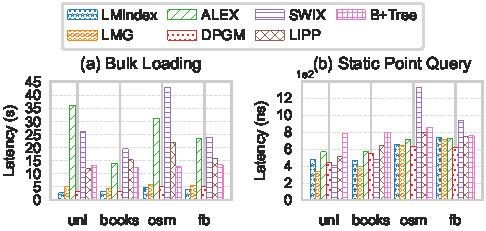
\includegraphics[width=1\textwidth]{vldbj_figs/bulk_purepq.pdf}
%         \caption{Bulk loading latency and static query latency.}
%         \label{fig:bulk_pquery}
%     \end{minipage}
%     \begin{minipage}[b]{0.49\textwidth}
%         \centering
%         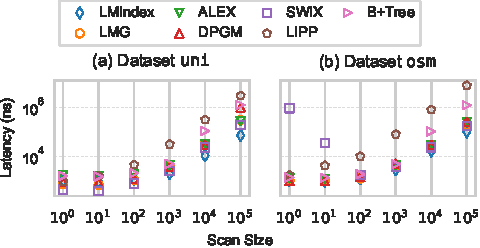
\includegraphics[width=1\textwidth]{vldbj_figs/pure_range_query.pdf}
%         \caption{Static range query latency under varying scan ranges.}
%         \label{fig:pure_rq}
%     \end{minipage}
% \end{figure*}

\subsection{Experimental Setup}
All code is implemented in C++ (available at \url{github.com/Nuiqv/LMIndex}). Our single-threaded experiments are conducted on an Ubuntu 24.04 machine with an AMD R9 7945HX 2.5GHz CPU and 64GB RAM, compiled with gcc -O3 -march=native.

\subsubsection{Baseline} We evaluate LMIndex and LMG against five representative baselines. Shared parameters such as the error threshold are aligned for fairness and others remain default to simulate real-world scenarios that are difficult to tune. (1) Dynamic PGM Index (DPGM) \cite{pgm20} is the update-capable variant of PGM, using the same error threshold~$\varepsilon$ as LMIndex. (2) ALEX~\cite{alex20} adopts gapped arrays with model-based insertion and exponential search. We set its max node size equal to our max layer size $\mathit{L}$. (3) SWIX~\cite{swix24} is optimized for streaming data with a flat routing layer and strong random access support. We use default settings. (4) STX B+Tree~\cite{stxbtree19} serves as the traditional baseline, evaluated with its default configuration. (5) LIPP \cite{lipp21, learned23} adopts a Zero Error strategy, which eliminates the need for error correction search steps during the query process. LMIndex is configured with a max layer size $\mathit{L}=2^{16}$, initial error threshold $\varepsilon=64$. LMG inherits the parameters of LM without employing an additional buffer; instead, it utilizes a gapped array with an expansion rate of $\tau=0.5$ to accommodate updates. This configuration is a balanced trade-off, and parameter sensitivity is discussed in Section~\ref{sec:param-eval}.

\subsubsection{Datasets}
All experiments are conducted on four representative datasets: a synthetic dataset with uniform distribution and three real-world datasets from the SOSD benchmark~\cite{sosd20}. The Uniform dataset (\texttt{uni}, 200M keys) contains keys drawn from a globally and locally linear distribution. The Amazon Books dataset (\texttt{books}, 200M keys) exhibits global non-linearity with partially linear local distributions. The Open Street Map dataset (\texttt{osm}, 200M keys) is both globally and locally non-linear. The Facebook user IDs dataset (\texttt{fb}, 200M keys) is mostly linear but includes a small number of large outliers. All keys are of the $64$-bit unsigned integer type and contain no duplicate values, consistent with prior studies or the open-source codebases of learned baselines.

% debug now
\subsubsection{Workloads}
We evaluate our approach primarily based on the following three categories of workloads. First, we consider static (read-only) workloads. For these scenarios, we perform read-only operations both immediately after bulk loading the entire dataset and after a specific volume of insertions. Second, we examine mixed read-write workloads, with the insertion frequencies set to 20\%, 40\%, 60\%, and 80\%, respectively. In these experiments, we initially bulk load 50\% of the data and subsequently execute 100M random read-write operations. Third, we evaluate range queries with lengths varying from $10^0$ to $10^5$. For these queries, we select 10K random starting keys and report the average latency. We evaluate LM exclusively under static scenarios. In addition, for point queries, we select 10M random keys and measure the latency.

\subsubsection{Metrics}
We measure time using average operation latency, recorded at nanosecond resolution with C++ \texttt{std::chrono}. Hardware-backed timers minimize instrumentation overhead to less than 5\%, rendering the interference with experimental results virtually negligible \cite{paoloni2010, najafi2021systems}. For memory, we track historical physical peak usage \texttt{VmHWM}. Unlike theoretical size, VmHWM represents the minimum spatial resources required for operation throughout the entire lifecycle. To ensure accuracy, all memory measurements subtract the initial usage before bulk loading.

\subsection{Evaluation of Diverse Dimensions}
We evaluated six key performance dimensions: bulk loading, point queries, range queries, stability, space usage, and updates. These dimensions characterize the fundamental lifecycle of an index, and critically impact its overall time-space efficiency.

\begin{figure*}
    \centering
    \begin{minipage}[b]{0.51\textwidth}
        \centering
        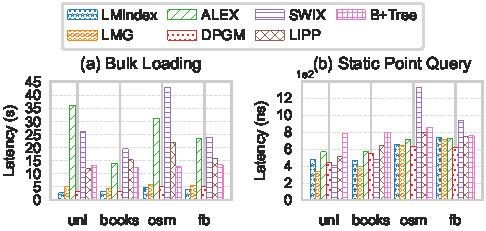
\includegraphics[width=1\textwidth]{vldbj_figs/bulk_purepq.pdf}
        \caption{Bulk loading latency and static query latency.}
        \label{fig:bulk_pquery}
    \end{minipage}
    \begin{minipage}[b]{0.47\textwidth}
        \centering
        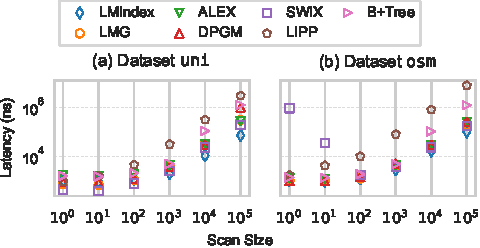
\includegraphics[width=1\textwidth]{vldbj_figs/pure_range_query.pdf}
        \caption{Static range query latency under varying scan ranges.}
        \label{fig:pure_rq}
    \end{minipage}
    \begin{minipage}[b]{1\textwidth}
        \centering
        \begin{subfigure}[b]{0.9\textwidth}
        \centering
        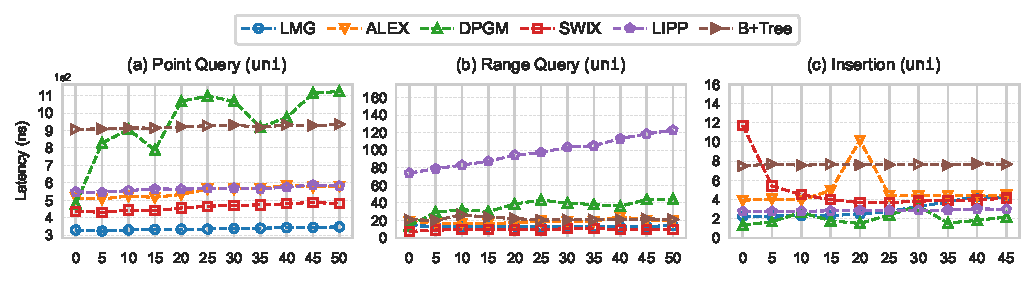
\includegraphics[width=1\textwidth]{vldbj_figs/stability_test_avg.pdf}
        \end{subfigure}
        \begin{subfigure}[b]{0.9\textwidth}
            \centering
            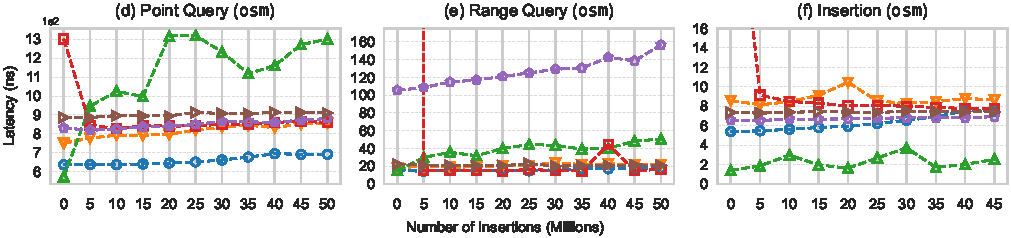
\includegraphics[width=1\textwidth]{vldbj_figs/stability_test_osm.pdf}
        \end{subfigure}
        \caption{Index stability and dynamic performance during continuous insertions (0-50M).}
        \label{fig:stability}
    \end{minipage}
\end{figure*}

% \begin{figure*}
%     \centering
%     \begin{subfigure}[b]{0.9\textwidth}
%     \centering
%     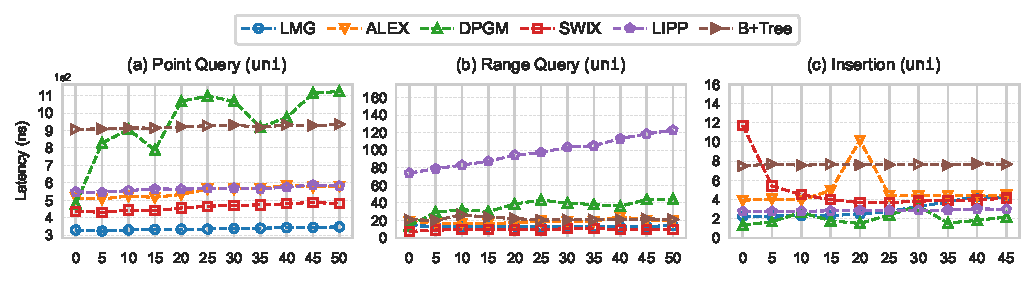
\includegraphics[width=1\textwidth]{vldbj_figs/stability_test_avg.pdf}
%     \end{subfigure}
%     \begin{subfigure}[b]{0.9\textwidth}
%         \centering
%         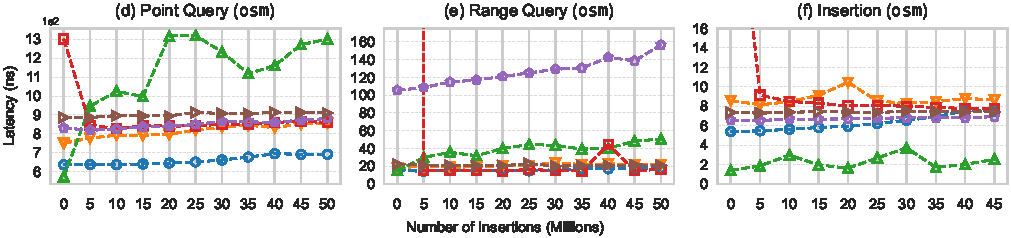
\includegraphics[width=1\textwidth]{vldbj_figs/stability_test_osm.pdf}
%     \end{subfigure}
%     \caption{Index stability and dynamic performance during continuous insertions (0-50M).}
%     \label{fig:stability}
% \end{figure*}

\subsubsection{Bulk Loading}
Bulk loading serves as a practical mechanism to initialize deployments and restore index quality after severe data distribution shifts. Figure \ref{fig:bulk_pquery}a reports the execution time across datasets, where our foundational structure, LMIndex, demonstrates superior initialization efficiency. Specifically, LMIndex achieves average speedups of 7.37$\times$ and 7.55$\times$ over top-down models like ALEX and SWIX, 4.37$\times$ over LIPP, 3.59$\times$ over B+Trees, and 1.14$\times$ over DPGM. Due to the gapped array allocation strategy, LMG slightly increases latency, being approximately 1.45$\times$ slower. Notably, the efficiency of both LMIndex and LMG does not exhibit drastic fluctuations across different data distributions.

The shared efficiency of LM and LMG inherently stems from the Bottom-Up training strategy. By greedily constructing segments through a single-pass scan over the sorted data ($O(N)$ complexity), our framework bypasses the expensive global data profiling required by other designs. Conversely, the structural bottlenecks of competing strategies become evident during initialization. Top-Down models (e.g., ALEX, SWIX) mandate recursive, multi-pass dataset scans to partition data and fit global models, resulting in significant loading delays. Similarly, Zero Error architectures like LIPP require the calculation and pre-allocation of a substantial number of contiguous empty slots, which diminishes bulk loading efficiency.

\subsubsection{Point Query}
\label{sec:point_query}
Point query execution time represents a fundamental metric for evaluating the retrieval efficiency of an index structure. Figure \ref{fig:bulk_pquery}b reports the static latency across read-only datasets. LMG demonstrates highly competitive retrieval performance, achieving average speedups of 1.30$\times$ over ALEX, 1.34$\times$ over LIPP, and 1.67$\times$ over B+Trees, while operating 1.15$\times$ faster than the base LMIndex. This baseline efficiency is primarily attributed to the Leaf-only Error strategy. By leveraging OETA to compress segment error thresholds, LMG further reduces error correction overhead, which is particularly effective on datasets with substantial latent compression potential (e.g., \texttt{uni}, \texttt{books}).

The performance differentiation becomes more pronounced under dynamic workloads with continuous insertions. As illustrated in the stability analysis (Figure \ref{fig:stability}a, \ref{fig:stability}d), competing architectures experience various degrees of performance degradation after 50M continuous insertions. For instance, DPGM, which exhibits static latency comparable to LMG, becomes 1.68$\times$ and 2.80$\times$ slower than LMG on the \texttt{osm} and \texttt{uni} datasets, respectively. In contrast, LMG sustains its point query efficiency throughout the dynamic lifecycle, extending its speedup over models like ALEX and LIPP to 1.63$\times$/1.23$\times$ and 1.68$\times$/1.28$\times$ on the \texttt{uni}/\texttt{osm}. The robustness and efficiency of point queries demonstrate that LM effectively maintains high indexing quality during updates.

\subsubsection{Range Query}
\label{sec:range_query}
In modern database systems, range queries serve as the foundational primitives for executing complex analytical operations, including relational joins and multi-dimensional aggregations (e.g., GROUP BY). Figure \ref{fig:pure_rq} reports the static range query latency across varying scan ranges (from $10^0$ to $10^5$). As anticipated, LMIndex exhibits the highest average range queries efficiency due to its strictly dense memory layout, executing slightly faster than LMG (1.13$\times$ faster). The gapped array allocation in LMG introduces a predictable, marginal overhead during sequential scans; nevertheless, LMG sustains a significant advantage over other architectures, achieving average speedups of 1.39$\times$ over ALEX, 1.30$\times$ over DPGM, and 2.54$\times$ over B+Trees. Crucially, zero error structures like LIPP incur a severe 11.41$\times$ slowdown compared to LMG. This execution penalty stems from the massive, dispersed empty slots required to enforce strict physical-to-prediction alignments, which heavily disrupt spatial locality and induce frequent cache misses during sequential traversals.

Regarding dynamic range queries, we evaluates the performance of $100$ range queries following continuous updates. As shown in Figure \ref{fig:stability}b, Figure \ref{fig:stability}e, indexes relying on fragmented experience notable performance degradation. Specifically, LIPP suffers a 7.65$\times$ slowdown on average due to progressive memory fragmentation. Similarly, DPGM (2.52$\times$ slowdown on average) experiences scan degradation because its LSM-tree style updates require traversing and merging data across multiple levels. Conversely, by leveraging efficient traversal of sequentially linked leaf nodes, B+Tree and ALEX are, on average, $1.48\times$ and $1.37\times$ slower, respectively. SWIX further strengthens its advantage through a completely flat segment indexing structure, outperforming LMG by $1.39\times$ on the \texttt{uni} dataset; however, it exhibits instability on the complex \texttt{osm} dataset, performing $1.86\times$ slower than LMG. LMG shares these structural advantages. The LM structure exhibits the characteristics of a flat array, while the segment list is ordered and linked similarly to a B+Tree. Consequently, LMG avoids severe fragmentation and the overhead of cross-level merging, ensuring both robustness and efficiency for range queries.

\begin{figure*}
    \centering
    \begin{minipage}[b]{0.32\textwidth}
        \centering
        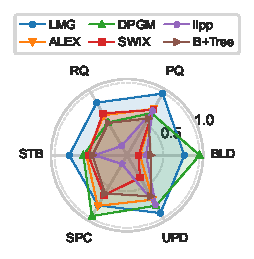
\includegraphics[width=1\textwidth]{vldbj_figs/radar.pdf}
        \caption{Comprehensive evaluation of multi-dimensional performance.}
        \label{fig:radar}
    \end{minipage}
    \begin{minipage}[b]{0.65\textwidth}
        \centering
        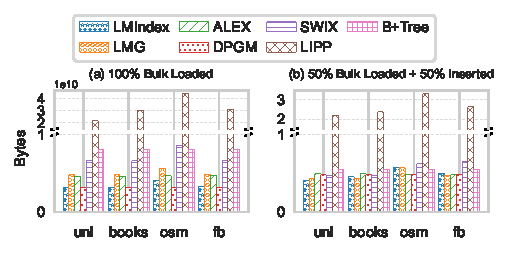
\includegraphics[width=1\textwidth]{vldbj_figs/space_test.pdf}
        \caption{Space footprint comparison under static initialization versus dynamic workload conditions.}
        \label{fig:space}
    \end{minipage}
    \begin{minipage}[b]{1\textwidth}
        \centering
        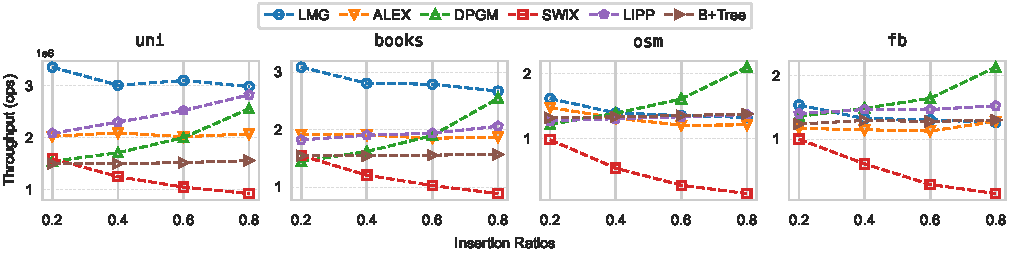
\includegraphics[width=1\textwidth]{vldbj_figs/update_test.pdf}
        \caption{Overall throughput under mixed read-write workloads with varying insertion ratios (0.2 to 0.8).}
        \label{fig:update}
    \end{minipage}
\end{figure*}

\subsubsection{Stability}
\label{sec:stability}
Maintaining performance stability during continuous updates is a fundamental capability for the long-term deployment of index structures. Figure \ref{fig:stability} trace the latency evolution of point queries, range queries, and insertions across a continuous insertion workload. As analyzed in Sections \ref{sec:point_query} and \ref{sec:range_query}, LMG demonstrates sustained read efficiency throughout the operational lifecycle. From a stability perspective, this confirms the structural robustness of the LM in dynamic scenarios, which additionally benefits from the inherent robustness of the underlying hybrid search.

Focusing on the insertion operations (Figure \ref{fig:stability}c, \ref{fig:stability}f), DPGM exhibits the lowest execution latency, operating at a 1.87$\times$ faster compared to LMG. This insertion efficiency directly derives from its LSM-Tree style update strategy, which sequentially buffers incoming records without querying for positioning. However, as established in previous sections, this mechanism inherently penalizes query performance. Conversely, traditional B+Trees maintain a highly stable insertion curve due to their standardized node-splitting mechanism, yet their absolute execution time remains consistently high, averaging a 1.94$\times$ slowdown relative to LMG. Other learned baselines, including ALEX, SWIX, and LIPP, record average execution slowdowns of 1.58$\times$, 1.84$\times$, and 1.04$\times$, respectively, placing LMG's overall insertion performance in a highly competitive position.

Furthermore, it can be observed that the insertion latency of LMG gradually increases during the later stages. This trend represents an expected structural phenomenon. Initially, the gapped array allocation efficiently absorbs incoming records. As the total data volume grows and the pre-allocated gaps reach capacity, the framework increasingly triggers local segment retrains. Consequently, the frequency of these retrains naturally scales with the data volume before eventually converging to a stable rate. Nevertheless, by strictly confining these necessary retrains to localized segments, LMG successfully balances insertion costs with robust long-term read efficiency.

\subsubsection{Space Usage}
Figure \ref{fig:space} reports the historical physical peak memory usage (\texttt{VmHWM}) under static and dynamic initialization scenarios. In the 100\% bulk loaded setting (Figure \ref{fig:space}a), the spatial footprint of LMG is 1.47x that of LMIndex on average. This value is very close to the theoretical expansion of the gapped array in LMG (i.e., $(1 + \tau = 1.5)\times$). This confirms the inherent space efficiency of the base LM architecture and indicates that LMG's spatial footprint is primarily dominated by its underlying gapped array. Among other baselines, DPGM exhibits the most compact static footprint (0.63$\times$) owing to its RMI-style structure (Only the model parameters need to be stored) and dense segment layout. ALEX operates at 0.93$\times$, while SWIX and B+Trees consume 1.40$\times$ and 1.60$\times$, respectively. As established in previous sections, LIPP incurs a massive 6.26$\times$ overhead due to the physical sparsity mandated by its zero error strategy.

The spatial dynamics shift notably under continuous insertions (Figure \ref{fig:space}b). Both DPGM and LMIndex see their relative space consumption increase to 1.02$\times$ compared to LMG, highlighting their spatial instability and the fragmentation costs incurred during continuous structural modifications. Crucially, while top-down architectures like ALEX can also employ gapped arrays to absorb updates, LMG ultimately consumes less space than ALEX (1.03$\times$), SWIX (1.17$\times$), and B+Trees (1.17$\times$). This advantage stems from the inherent space efficiency of the foundational LM structure, which naturally naturally fits the underlying segment distribution and does not require a lot of routing metadata. LIPP remains highly inefficient at 5.48$\times$. Consequently, LMG's structural design effectively prevents severe memory inflation throughout its lifecycle.

\subsubsection{Update Performance}
Distinct from the stability evaluated in Section \ref{sec:stability}, this section assesses index throughput under mixed workloads, with write ratios varying from 0.2 to 0.8. Averaged across all datasets and workload configurations, LMG demonstrates highly competitive overall throughput, operating 1.31$\times$ faster than ALEX, 1.49$\times$ over B+Trees, 1.19$\times$ over LIPP, 1.26$\times$ over PGM, and 3.50$\times$ over SWIX. Specifically, LMG consistently achieves the highest throughput on the \texttt{uni} and \texttt{books} datasets, validating its efficiency under these distributions.

On the \texttt{osm} and \texttt{fb} datasets, LMG slightly trails DPGM and LIPP under specific mixed workloads. This performance variance is primarily driven by the distinct structural characteristics of the baselines. For example, the LSM-tree-style buffer in DPGM enables direct insertions without requiring query routing; however, distributing data across multiple levels degrades the efficiency of subsequent reads. Furthermore, LMG exhibits a slight throughput reduction under specific heavy-read workloads. This behavior stems from our conservative segment retraining strategy. To strictly guarantee read efficiency and preserve local error bounds, LMG proactively triggers segment retrains before the pre-allocated gaps are fully exhausted. While this deliberate architectural trade-off introduces a predictable structural overhead as write operations occur, it successfully ensures bounded, long-term operational stability without compromising read performance.

\subsubsection{Holistic Performance and Multi-dimensional Balance}
Figure \ref{fig:radar} synthesizes the holistic performance of the evaluated indexes through a normalized radar chart (score from 0.0 to 1.0). For most dimensions (e.g., Bulk Loading and Space Usage), normalized scores are derived by averaging relative performance metrics across all datasets. To accurately capture long-term index stability, the Stability (STB) dimension is quantified using the Area Under the Curve (AUC), defined as $AUC = \int_{0}^{50M} Latency(x) \,dx$. This formulation effectively penalizes unpredictable latency spikes and sustained execution delays over the continuous insertion lifecycle. Furthermore, the Point Query (PQ) and Range Query (RQ) dimensions aggregate both static and dynamic workloads from STB to reflect a comprehensive operational lifecycle.

The resulting visualization exposes the severe multi-dimensional trade-offs inherent in existing baselines. For instance, while DPGM achieves near-optimal normalized scores in Bulk Loading (1.000) and Space Consumption (0.969), its structural rigidity severely penalizes its Range Query (0.520) and Stability (0.602) performance. Similarly, zero error architectures like LIPP catastrophically compromise Space (0.141) and Range Queries (0.148) to maintain read limits. In contrast, LMG yields the most expansive and balanced performance polygon. By consistently sustaining high normalized scores across all six dimensions (ranging from 0.789 to 0.981), LMG empirically validates its core design philosophy: avoiding catastrophic degradation in any single metric to deliver robust, general-purpose efficiency across diverse and dynamic database workloads.

\begin{figure*}
    \centering
    \begin{minipage}[b]{0.5\textwidth}
        \centering
        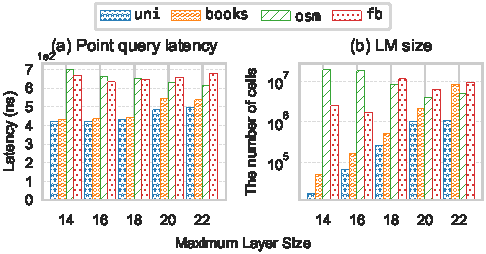
\includegraphics[width=\linewidth]{vldbj_figs/max_layer_size.pdf}
        \caption{Evaluation of point query performance and LM size under different maximum layer sizes ($2^{14}$ to $2^{22}$) for LM.}
        \label{fig:max_layer_size}
    \end{minipage}
    \begin{minipage}[b]{0.48\textwidth}
        \centering
        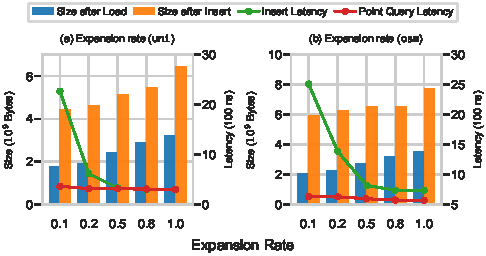
\includegraphics[width=1\textwidth]{vldbj_figs/expansion_rate.pdf}
        \caption{Impact of expansion rate on LMG in terms of point query, insert and space.}
        \label{fig:expansion_rate}
    \end{minipage}
    % \hfill
    \begin{minipage}[b]{0.27\textwidth}
        \centering
        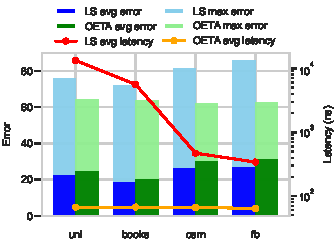
\includegraphics[width=\linewidth]{vldbj_figs/oeta_vs_ls.pdf}
        \caption{Analysis of OETA and Least Squares.}
        \label{fig:oeta_vs_ls}
    \end{minipage}
    \begin{minipage}[b]{0.27\textwidth}
        \centering
        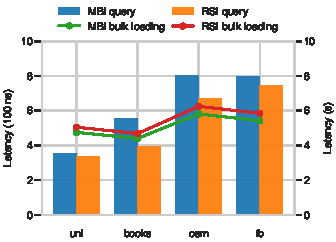
\includegraphics[width=\linewidth]{vldbj_figs/lmg_insert_comparison.pdf}
        \caption{Comparison of gap allocation strategies.}
        \label{fig:lmg_insert_comparison}
    \end{minipage}
    % \hfill
    \begin{minipage}[b]{0.45\textwidth}
        \centering
        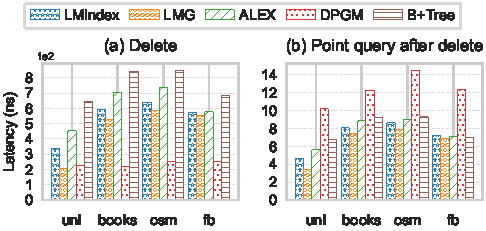
\includegraphics[width=0.86\linewidth]{vldbj_figs/delete_test.pdf}
        \caption{Deletion efficiency and its impact on query performance.}
        \label{fig:delete_test}
    \end{minipage}
\end{figure*}

\subsection{Detailed Evaluation}
\subsubsection{Parameter Evaluation}
\label{sec:param-eval}
We evaluate the impact of the maximum layer size $\mathit{L}$ on LMIndex, as well as the expansion rate $\tau$ on LMG.

\textbf{Max Layer Size.} Figure \ref{fig:max_layer_size} evaluates the sensitivity of the LM structure to its maximum layer size $\mathit{L}$ (from $2^{14}$ to $2^{22}$). Crucially, point query latency exhibits relative consistency across all $\mathit{L}$ values, demonstrating that retrieval efficiency is structurally robust and insensitive to parameter tuning. Regarding space usage, the size of LM remains relatively stable for complex data distributions (e.g., \texttt{books}, \texttt{osm}, and \texttt{fb}). Conversely, on the relatively linear and uniform dataset \texttt{uni}, expanding $\mathit{L}$ increases the number of cells per segment, leading to a significant increase in index size. However, despite this trend, the absolute LM size on the \texttt{uni} dataset remains the lowest among all evaluated distributions, and it stabilizes within the $2^{20}$ to $2^{22}$ parameter range. Overall, adjusting $\mathit{L}$ across a vast parameter space achieves relatively stable performance; a smaller $\mathit{L}$ can yield a slight advantage on more linear distributions, though the absolute magnitude of this improvement is marginal (compare to complex distributions). This further verifies the structural robustness of LM.

\textbf{Expansion Rate.} The expansion rate $\tau$ determines the proportion of reserved gaps in the data array, influencing both memory footprint and update/query performance. As shown in Figure \ref{fig:expansion_rate}, increasing $\tau$ initially reduces insertion latency, but the benefits saturates once most updates are absorbed by existing gaps. Query latency also improves slightly due to fewer correction steps, though the gain quickly saturates, especially on datasets with linear distributions like \texttt{uni}. Meanwhile, memory usage rises steadily with larger $\tau$, reflecting the overhead of excess reserved gaps. Therefore, selecting $\tau$ requires balancing update performance against memory overhead. Overall, the magnitude of $\tau$ is linearly correlated with space consumption. Regarding queries, the impact of $\tau$ remains relatively stable; for insertions, a smaller $\tau$ is preferable. However, we identify $0.5$ as a ``sweet spot'': across two datasets with vastly different distributions, it serves as the inflection point where the slope of insertion latency begins to flatten, while still maintaining a moderate spatial footprint.

\subsubsection{Gap Allocation Strategy}
We compare two gap allocation strategies within LMG: model-based insertion \cite{alex20} and reserved-space insertion. As shown in Figure \ref{fig:lmg_insert_comparison}, the reserved-space insertion incurs slightly higher bulk load time due to more complex gap placement. However, it consistently delivers better query performance by pre-allocating gaps more evenly across array. This reduces average correction length and improves search performance. Overall, given the efficient bulk loading process of LMG, the small increase in load time is an acceptable trade-off for stronger runtime performance.

\subsubsection{OETA vs. Least Squares} 
\label{sec:oeta_vs_ls}
% We compare OETA with the classic least squares (LS) method across three metrics: average maximum error per segment, average mean error per segment, and algorithm runtime. As shown in Figure \ref{fig:oeta_vs_ls}, OETA outperforms LS by reducing the average maximum error by 15.4\%–26.6\% while incurring only 0.5\%–18\% of LS’s runtime. These improvements align with OETA's theoretical design, which directly minimizes the maximum segment error to accelerate binary search. Moreover, this efficiency makes OETA suitable for time-sensitive scenarios, offering an alternative approach to computing model parameters for other learned indexes.

We evaluate the training efficacy of OETA against the standard least squares (LS) baseline by measuring three key metrics: average maximum error per segment, average mean error per segment, and algorithm runtime. As shown in Figure \ref{fig:oeta_vs_ls}, OETA consistently yields tighter error bounds. Compared to the LS baseline, OETA improves the average mean error by 12.5\% on average and reduces the average maximum error by 15.4\% to 26.6\%. This mean/maximum error trade-off is particularly effective when we employ maximum error sensitive binary search. In terms of runtime, OETA demonstrates fundamental advantages in computational efficiency and stability. Experimental results indicate that OETA consumes only 0.5\% to 18\% of the runtime required by LS. Crucially, while the performance of the Least Squares (LS) method exhibits high variance, OETA maintains a nearly consistent low overhead across diverse data distributions. The experimental results manifest the characteristics of an $O(1)$ algorithm, aligning with our theoretical derivations. Furthermore, this efficiency renders OETA more suitable for time-sensitive scenarios, providing an alternative approach for computing model parameters in other learned indexes.

\begin{table}
  \caption{Statistics of Linear Map}
  \small
  \begin{tabular}{lcccc}
  % \begin{tabular}{lllll}
    \toprule
     &\textbf{uni}&\textbf{books}&\textbf{osm}&\textbf{fb}\\
    \midrule
    \textbf{Avg update latency (ns)}	& 156.86 & 159.99 & 280.13 & 111.05\\
    \textbf{Avg layer size}			& 61504	&671.6	&3333	&20.4\\
    \textbf{Avg search depth}			& 0	&0.004	&0.989	&2.184\\
    \textbf{Avg segment's cells}			& 4.7	&5.6	&135.4	&3.6\\
    \textbf{Max layer depth}			& 0	&2	&2	&3\\
    \textbf{Num of layer} 			& 1	&249	&15704	&93025\\
    \textbf{LM building time / total}	    & 0.02\% & 0.16\% & 6.16\% & 3.08\%\\
    \textbf{LM space usage / total}	    & 0.066\% & 0.17\% & 15.7\% & 1.73\%\\
  \bottomrule
  \label{tab:lm_info}
\end{tabular}
\end{table}
\subsubsection{Linear Map Evaluation} 
\label{sec:lm_eval}
Table \ref{tab:lm_info} presents key statistics of LM, except update latency measured under a 50\% random insertion workload and all other metrics collected after fully loading each dataset. The root layer is defined as depth 0. Across datasets, LM exhibits consistently low and stable update latency. Most keys are located within 1 layer, with the \texttt{fb} dataset being an exception due to the segments containing a small number of large outliers placed at the root. Owing to the flat layer structure and the training-free model design, LM achieves almost negligible build time, accounting for just 0.02\%–6.16\% of total index construction time.


\subsubsection{Delete Evaluation}
Figure \ref{fig:delete_test} evaluates the deletion efficiency by removing 50\% of the dataset and measuring the subsequent point query latency. In terms of sheer deletion speed, DPGM exhibits the lowest latency. This efficiency derives directly from its LSM-tree-style mechanism, which rapidly appends tombstone markers without verifying the actual existence of the target keys. However, this blind insertion strategy inevitably penalizes subsequent read operations, causing DPGM to perform 2.05$\times$ slower than LMG in post-deletion queries on average. Conversely, LMG employs a more balanced approach that combines in-place tombstone marking with localized segment merging and retraining. While this structural maintenance introduces a slight latency overhead during the deletion phase (though LMG still operates 1.45$\times$ and 1.85$\times$ faster than ALEX and B+Trees, respectively), it effectively bounds the deterioration of prediction accuracy. Ultimately, LMG strikes a robust architectural trade-off, efficiently accommodating massive deletions while preserving long-term query stability.

\section{Discussion and Extensibility}
\label{sec:extend}
While the current LMG architecture is fundamentally designed as a foundational framework to achieve multi-dimensional performance balance for complex workloads, its highly decoupled hybrid structure remains inherently extensible. By isolating the routing logic from the underlying physical data layout, LMG provides a versatile blueprint capable of supporting a broader spectrum of complex database operations and query paradigms.

\textbf{Duplicate Keys Support.} LMG could naturally accommodate duplicate keys by pushing the handling logic down to the localized segments. In this configuration, the upper-level LM structure would solely manage segment distribution information, remaining entirely oblivious to key duplication. During the localized model training phase, the segment would train its model exclusively on unique keys and their physical positions, thereby ensuring prediction accuracy and bounding inference errors. Consequently, point queries could efficiently locate the target primary key within the local segment, and subsequent range scans could seamlessly traverse the associated value lists without disrupting the contiguous segment alignment.

\textbf{Concurrent Operations.} To support multi-threaded database workloads, LMG could integrate standard concurrency control protocols. Because structural modifications (SMOs), such as gap allocation and segment retraining, are strictly confined to local boundaries within our hybrid architecture, LMG would be well-suited to employ fine-grained, segment-level latching (e.g., read-write locks) for the bottom data layer. This localized absorption would drastically minimize lock contention during highly concurrent insertions. Simultaneously, the upper routing layer could be protected using Optimistic Concurrency Control (OCC) or versioned locks, ensuring that read transactions traverse the hierarchy without heavy synchronization overheads.

\textbf{Vector and High-Dimensional Queries.} Although originally optimized for 1D scalar keys, LMG could be adapted to support high-dimensional vector searches. This extension could be achieved by employing order-preserving mappings, such as Space-Filling Curves (e.g., Z-order or Hilbert curves) or Locality-Sensitive Hashing (LSH), to project multi-dimensional vectors into single-dimensional scalar keys. LMG could subsequently be constructed over these mapped keys. Under this paradigm, complex high-dimensional proximity evaluations or $k$-nearest neighbor ($k$-NN) candidate retrievals would effectively be transformed into localized 1D range scans, allowing the system to leverage LMG's robust sequential scanning efficiency.

\section{Related Work}
\label{sec:rel-work}
% \subsection{Learned Index}
% Learned indexes leverage the linearity of data distributions to map keys to possible positions, and this can be achieved using a non-linear model \cite{case18, cdfshop20, lipp21} or a piecewise linear model \cite{radixspline20, xindex20, madex20}. Currently, most learned indexes employ PLM to predict positions due to the simplicity of linear model parameters and the efficiency of training. In addition, some experiments have shown their effectiveness in various real-world datasets \cite{sosd20}. Moreover, learned indexes have also been extended to handle multimodal data, including one-dimensional key-value pairs \cite{pgm20, alex20, swix24, shift21}, high-dimensional vectors \cite{flood20, Tsunami20, coax23, learnedaknn22}, string data \cite{sindex20, rss21, lits24}, spatial data \cite{ifx20, lisa20, wisk23}, and more.

% \textbf{Segment Index:} In PLM-based learned indexes, the higher-level segment index plays a crucial role in overall performance. The RMI structure \cite{case18, pgm20} recursively constructs multilayer models by gradually magnifying the precision constraint to route to the underlying data. The tree-based hierarchical structure \cite{alex20, lipp21} divides and constructs the hierarchy more rapidly, and the lower coupling between layers allows local updates without training the entire model. In recent years, some learned indexes \cite{finedex21, swix24} have introduced flat structures to significantly reduce the depth of the routing by expanding the size of a single layer, but still require model training for efficient routing of elements within the layer. We propose the LM structure to address this issue. By computing the mapping parameters of elements, LM can locate any element within a flat layer with $O(1)$ cost without training a model, while also enabling efficient local updates.

% \textbf{Piecewise Linear Model}: Another major focus of current learned indexes is training PLM. PLM training can be divided into segmentation and regression. In segmentation, existing work either takes top-down approaches \cite{case18, alex20, swix24, carmi22} or bottom-up approaches \cite{fiting-tree19, pgm20, bourbon20}. The top-down method allows for fine-tuning the segments as a whole, such as SWIX \cite{swix24}, which uses second-order derivatives for segmentation to make the distribution within segments more linear. In contrast, the bottom-up approach segments the data in a data-driven manner based on certain constraints. PGM \cite{pgm20} introduces the \cite{line81} algorithm to ensure the minimum number of segments under a given error threshold constraint. In regression, \cite{alex20, sindex20, finedex21, swix24} employ the least squares method to minimize the average error, while \cite{pgm20, madex20, towards21} compute the linear parameters quickly by finding one line of the convex hull. LMIndex adopts a bottom-up approach to ensure the optimal number of segments and further utilizes OETA to efficiently obtain the linear parameters with the smallest maximum error within each segment.

% % \subsection{In-memory Index}
% % Tree-based in-memory indexes \cite{btree06, btree11, bwtree13} are mainstream techniques in traditional database systems. Index structures are organized in a tree-like manner, requiring significant memory and supporting both range and point queries. However, when indexing large data, as the tree depth increases and access paths grow, performance degradation can occur due to pointer chasing and cache misses. Hash-based in-memory indexes \cite{dynamichash98, hash16} excel in point query scenarios but lack efficient range query support, and hash collisions may lead to performance degradation. Hybrid index structures, such as LSM-tree \cite{lsmtree96, lsmtree17, remix21} and adaptive indexes \cite{adaptive18, adaptive22}, combine the advantages of various indexing techniques, adapting to different workloads. However, these structures are often more complex and have a narrower range of applicability.

\textbf{Evolution of Learned Indexes.}
The paradigm of learned indexing was pioneered by RMI \cite{case18}, which leverages the cumulative distribution function (CDF) of underlying data to map search keys to approximate physical locations. While early model-based indexes \cite{radixspline20, plex21, shift21} primarily targeted static workloads, the inherent limitations of read-only structures in dynamic environments spurred the development of updatable architectures. FITing-Tree \cite{fiting-tree19} and PGM \cite{pgm20} introduced bottom-up construction strategies governed by strict error bounds. Conversely, ALEX \cite{alex20} expanded upon the RMI concept by employing a top-down, data-driven construction that deliberately sacrifices structural balance to achieve superior model fitting across varying data granularities. These foundational works triggered a rapid proliferation of learned index designs, establishing a vast design space characterized by distinct structural layouts and optimization objectives.

\textbf{Structural Paradigms.}
The underlying routing architecture fundamentally dictates the search efficiency and update capability of a learned index. Hierarchical models typically employ either recursive, multi-layer error bounds \cite{case18, pgm20} or tree-based layouts \cite{alex20, lipp21} to iteratively refine position estimates. While tree-based designs facilitate localized updates without requiring holistic model retraining, the cascading traversal overhead remains non-trivial. Recent advancements \cite{uplif25, swix24, cabin24} advocate for flattened structures, deliberately reducing routing depth by expanding the capacity of individual layers. However, navigating these expansive layers still demands computational overhead for model inference. In contrast, our proposed LM structure addresses this bottleneck by computing deterministic mapping parameters. This enables $O(1)$ intra-layer routing without continuous model retraining, inherently supporting efficient local modifications while maintaining high accuracy.

\textbf{Model Construction and Optimization.}
Another critical dimension in learned index design is the methodology used for data segmentation and linear approximation. Segmentation strategies broadly bifurcate into top-down \cite{case18, alex20, swix24, carmi22} and bottom-up \cite{fiting-tree19, pgm20, bourbon20} frameworks. Top-down methodologies optimize segments holistically; for instance, SWIX \cite{swix24} utilizes second-order derivatives to enforce tighter linearity within segments. Conversely, bottom-up algorithms generate data-driven partitions governed by strict error thresholds. Within these segments, the regression techniques vary significantly: several frameworks optimize for average error using least squares \cite{alex20, sindex20, finedex21, swix24}, while others compute bounding parameters via convex hull algorithms to guarantee maximum error bounds \cite{pgm20, madex20, towards21}. Model retraining also incurs significant tail latency, a challenge that several studies \cite{chameleon24, vega25, hire25} have attempted to mitigate. Building upon these foundations, LMIndex leverages a bottom-up segmentation strategy coupled with the OETA algorithm to efficiently derive parameters that strictly minimize the maximum error per segment. Furthermore, this can be further refined through advanced parameter tuning \cite{tuning22, airindex23, newtuning25} and dynamic statistics maintenance \cite{sali23}.

\textbf{Expanding Modalities and Hardware Utilization.}
Beyond one-dimensional numeric keys, the learned index design space has diversified to accommodate complex data types. Researchers have tailored models for multi-dimensional vectors \cite{flood20, Tsunami20, coax23, learnedaknn22}, string data \cite{sindex20, rss21, lits24}, spatial datasets \cite{ifx20, lisa20, wisk23}, and streaming windows \cite{flirt23}. Concurrently, orthogonal optimizations have emerged to exploit modern hardware topologies, including CPU cache optimization \cite{carmi22}, GPU acceleration \cite{hyper24}, concurrent execution \cite{xindex20, finedex21}, and persistent memory efficiency \cite{apex21, simple23, learnedpmem23, disklearned24, wipe24, making24}. Despite these specialized advancements, balancing high-dimensional performance with robust, dynamic updatability remains an ongoing challenge in the field.


\section{Conclusions}
\label{sec:conclusions}
% This paper introduces the lightweight and efficient model index structure Linear Map (LM) and the Optimal Error Threshold Algorithm (OETA), which together form LMIndex and its variant, LMG (LMIndex with gaps). Experimental results show that LMIndex is well-suited for space-constrained read-heavy workloads. And LMG outperforms B+Tree across six key evaluation dimensions and achieves the best overall performance compared to other baselines, demonstrating its potential to become a universal index for complex real-world scenarios.

% This work introduces Linear Map (LM), a lightweight and model-indexing architecture, together with the Optimal Error Threshold Algorithm (OETA). 
% These components jointly form LMIndex and its enhanced variant LMG. LMIndex is suitable for space-constrained read-heavy workloads. Meanwhile, LMG extends LMIndex with adaptive gap allocation and hybrid correction, delivering superior update performance and stability. Across six practical evaluation dimensions, LMG achieves the best overall performance.

This paper introduces a lightweight decoupled model-indexing structure and the Optimal Error Threshold Algorithm (OETA) as foundational mechanisms for highly efficient learned indexing. By integrating these core components, we propose LMG, a robust learned index framework. Extensive evaluations across six practical dimensions demonstrate that LMG mitigates inherent performance tradeoffs, maintaining efficiency and multi-dimensional stability.

% This paper introduces a lightweight decoupled model-indexing structure and the Optimal Error Threshold Algorithm (OETA) as foundational mechanisms for highly efficient learned indexing. By integrating these core components, we propose LMG, a robust indexing framework explicitly tailored for dynamic workloads. To effectively manage data distribution shifts and insertion turbulence, LMG further incorporates an adaptive gap allocation strategy. Extensive evaluations across six practical dimensions demonstrate that this unified architecture successfully mitigates the performance tradeoffs inherent in recent baselines. Ultimately, LMG maintains competitive read/write efficiency and structural stability, delivering a comprehensively balanced indexing solution.







% \section{Introduction}
% \label{intro}
% Your text comes here. Separate text sections with
% \section{Section title}
% \label{sec:1}
% Text with citations \cite{lisa20} and.
% \subsection{Subsection title}
% \label{sec:2}
% as required. Don't forget to give each section
% and subsection a unique label (see Sect.~\ref{sec:1}).
% \paragraph{Paragraph headings} Use paragraph headings as needed.
% \begin{equation}
% a^2+b^2=c^2
% \end{equation}

% % For one-column wide figures use
% \begin{figure}
% % Use the relevant command to insert your figure file.
% % For example, with the graphicx package use
%   \includegraphics{example.eps}
% % figure caption is below the figure
% \caption{Please write your figure caption here}
% \label{fig:1}       % Give a unique label
% \end{figure}
% %
% % For two-column wide figures use
% \begin{figure*}
% % Use the relevant command to insert your figure file.
% % For example, with the graphicx package use
%   \includegraphics[width=0.75\textwidth]{example.eps}
% % figure caption is below the figure
% \caption{Please write your figure caption here}
% \label{fig:2}       % Give a unique label
% \end{figure*}
% %
% % For tables use
% \begin{table}
% % table caption is above the table
% \caption{Please write your table caption here}
% \label{tab:1}       % Give a unique label
% % For LaTeX tables use
% \begin{tabular}{lll}
% \hline\noalign{\smallskip}
% first & second & third  \\
% \noalign{\smallskip}\hline\noalign{\smallskip}
% number & number & number \\
% number & number & number \\
% \noalign{\smallskip}\hline
% \end{tabular}
% \end{table}


%\begin{acknowledgements}
%If you'd like to thank anyone, place your comments here
%and remove the percent signs.
%\end{acknowledgements}

% BibTeX users please use one of
% \bibliographystyle{spbasic}      % basic style, author-year citations
\bibliographystyle{spmpsci}      % mathematics and physical sciences
% \bibliographystyle{spphys}       % APS-like style for physics

% \bibliography{lm_reference}   % name your BibTeX data base
% \bibliography{new_references}   % name your BibTeX data base
\bibliography{cleaned_references}   % name your BibTeX data base

\end{document}
% end of file template.tex

